\documentclass[ignorenonframetext,xcolor=x11names]{beamer}

\definecolor{mun}{RGB}{134,38,51}
\definecolor{mun2}{RGB}{99,102,106}
%\definecolor{mun}{cmyk}{0,.3922,.2392,.1686}
\definecolor{code}{RGB}{0, 0, 128}
\definecolor{code}{gray}{0.95}

\mode<presentation>
{
%  \usetheme{boxes}
%  \usetheme{default}
%  \usetheme{Montpellier}
%  \usetheme{Singapore}
%   \usetheme{Rochester}
%  \usecolortheme{crane}
%  \usecolortheme{dolphin}
%  \usecolortheme{lily}
%  \usecolortheme{orchid}
  \usecolortheme{rose}
  \setbeamercovered{transparent}
%  \usefonttheme[onlymath]{serif}
  \setbeamercolor*{structure}{bg=mun,fg=mun}
  \setbeamercolor*{palette primary}{use=structure,fg=white,bg=structure.fg}
  \setbeamercolor*{palette secondary}{use=structure,fg=white,bg=structure.fg}
  \setbeamercolor*{palette tertiary}{use=structure,fg=white,bg=black}
  \setbeamercolor*{palette quaternary}{fg=white,bg=black}
  \setbeamercolor{section in toc}{fg=black,bg=white}
  \setbeamercolor{alerted text}{use=structure,fg=structure.fg!50!black!80!black}
  \setbeamercolor{titlelike}{parent=palette primary,fg=structure.fg!50!black}
  \setbeamercolor{frametitle}{bg=mun,fg=white}
  \setbeamercolor*{titlelike}{parent=palette primary}

  \setbeamercolor{normal text}{fg=black!90}
  \setbeamercolor{math text}{fg=black}
  \setbeamercolor{quote}{bg=gray!20}
  \setbeamercolor{quotation}{bg=gray!20}
  \setbeamerfont{cite}{size=\scriptsize}
  \setbeamerfont{quote}{size=\footnotesize}
  \setbeamerfont{quotation}{size=\footnotesize}
  \setbeamercolor{red text}{fg=red!75!black}
  \setbeamertemplate{bibliography item}[triangle]
  \setbeamertemplate{enumerate item}[square]
  \setbeamertemplate{blocks}[rounded][shadow=true]
  \setbeamertemplate{navigation symbols}{}
  \setbeamertemplate{footline}[frame number]
}
\usepackage{tcolorbox}
\usepackage{amsmath}
\usepackage{physics}
\usepackage{pgf}
\usepackage[english]{babel}
\usepackage[latin1]{inputenc}
\usepackage{times}
\usepackage[T1]{fontenc}
\usepackage{multicol}
\usepackage{multirow}
\usepackage{fancyvrb}
\usepackage{tabularx}
\usepackage{amsmath}
\usepackage{bbm}
\usepackage{alltt}
\usepackage{hyperref}
\hypersetup{
    colorlinks=true,
    linkcolor=blue,
    filecolor=magenta,      
    urlcolor=blue,
}
\usepackage{minted}
\newminted{cypher}{autogobble,bgcolor=code,breakbytoken,frame=single,framesep=3pt}
\newminted{R}{autogobble,bgcolor=code,breakbytoken,frame=single,framesep=3pt}
\newminted{text}{autogobble,bgcolor=code,breakbytoken,frame=single,framesep=3pt}
\newminted{sql}{autogobble,bgcolor=code,breakbytoken,frame=single,framesep=3pt}
\newminted{bash}{autogobble,bgcolor=code,breakbytoken,python3,frame=single,framesep=3pt}
\newminted{xml}{autogobble,bgcolor=code,breakbytoken,python3,frame=single,framesep=3pt}
\newminted{python}{bgcolor=code,breakbytoken,python3,frame=single,framesep=3pt}
\newminted{html}{autogobble,bgcolor=code,breakbytoken,frame=single,framesep=3pt}
\newminted{js}{autogobble,bgcolor=code,breakbytoken,frame=single,framesep=3pt}
\AtBeginEnvironment{minted}{%
  \renewcommand{\fcolorbox}[4][]{#4} \scriptsize}
\AtEndEnvironment{minted}{%
  \normalsize}

%\newcommand{\Pr}{\operatorname{Pr}}
\newcommand{\argmax}{\operatorname*{argmax}}
\newcommand{\argmin}{\operatorname*{argmin}}
\newcommand{\Ident}{\operatorname{I}}

\author % (optional, use only with lots of authors)
{Joerg Evermann}
% - Give the names in the same order as the appear in the paper.
% - Use the \inst{?} command only if the authors have different
%   affiliation.

\institute%[Universities of Somewhere and Elsewhere] % (optional, but mostly needed)
{
  Faculty of Business Administration\\
  Memorial University of Newfoundland \\ 
  \texttt{jevermann@mun.ca} 
}

\date{}

\pgfdeclareimage[width=1.5cm]{university-logo}{../MUN_LOGO_CMYK}
\logo{\pgfuseimage{university-logo}}

% If you wish to uncover everything in a step-wise fashion, uncomment
% the following command: 

%\beamerdefaultoverlayspecification{<+->}

 
\title{Business 4720 - Class 7}

\subtitle{Data Visualization with R}

\begin{document}

\begin{frame}{}
  \titlepage
  \footnotesize 
  \begin{center}

\includegraphics[height=.5in]{../by-nc.png}

Unless otherwise indicated, the copyright in this material is owned by Joerg Evermann. This material is licensed to you under the \href{https://creativecommons.org/licenses/by-nc/4.0/}{Creative Commons by-attribution non-commercial license (CC BY-NC 4.0)}
\end{center}
 
  
XKCD comics are copyright by their creator (\url{www.xkcd.com}) and licensed under CC-BY-NC
\end{frame}

\begin{frame}{This Class}

\begin{block}{What You Will Learn:}
\begin{itemize}
  \item Introduction to Visualization
  \item Visualizing data with R using the ggplot2 library
\end{itemize}
\end{block}
\end{frame}


\begin{frame}{Why Visualize?}
  \begin{quote} \large \centering
    ''A Picture is Worth 1000 Words''
  \end{quote}
  
\begin{itemize}
  \item Humans are good at visual pattern recognition, but
  \begin{itemize}
    \item Humans also identify patterns where there are none!
    \item It's easy to mislead or deceive with visualization (others and oneself!)
  \end{itemize}
\end{itemize}
\end{frame}

\begin{frame}{Why Visualize?}
\begin{block}{Visual Discovery: Sense Making}
  \begin{itemize}
  \item \alert{Exploration}, confirmation or verification
  \item Iterative, dynamic
  \end{itemize}
\end{block}

\begin{block}{Declarative Visualization: Storytelling}
  \begin{itemize}
  \item \alert{Explanation}
  \item Affirming, convincing
  \item Presenting, explaining
  \item Decision support
  \item Static
  \end{itemize}
\end{block}

\begin{block}{Operational Visualization: Monitoring}
	\begin{itemize}
		\item Supervision, alarms
		\item Operational decision making
	\end{itemize}
\end{block}
\end{frame}

\begin{frame}{Purpose of Visualization}
\begin{itemize}
  \item Simplify, summarize \& abstract
  \item Compare
  \item Identify trends, patterns \& relationships
  \item Gain insights
\end{itemize}
\end{frame}

\begin{frame}{Quantitative Messages}
\begin{enumerate}
   \item Time-series (e.g. line chart)
   \item Ranking (e.g. bar chart)
   \item Part-whole (e.g. pie chart)
   \item Deviation (e.g. bar chart)
   \item Frequency distribution (e.g. histogram, boxplot)
   \item Correlation (e.g. scatter plot)
   \item Nominal comparison (e.g. bar chart)
   \item Geographic distribution (e.g. cartogram)
\end{enumerate}
\end{frame}

\begin{frame}{Honesty in Visualization}
\begin{block}{General Guidelines}
	\begin{itemize}
		\item Do not deceive your target audience
		\item Do not diminish or hide relationships or trends
		\item Do not exaggerate relationships or trends
		\item Do not confuse or obfuscate
	\end{itemize}
\end{block}
\end{frame}

\begin{frame}{Honesty in Visualization}
\begin{block}{Specific ''no-nos''}
	\begin{itemize}
		\item Graph unrelated data to suggest non-existent relationships
		\item Scale multiple vertical axes to suggest correlations
		\item Truncate or scale axes to hide or exaggerate trend
		\item Scale in multiple dimensions
		\item Plot cumulative growth to hide trend
		\item Use maps for non-geographic data
		\item Use incomplete data (''cherry-picking'')
		\item Use invalid data
	\end{itemize}	
\end{block}
\end{frame}

\begin{frame}{Label your Axes (XKCD)}
  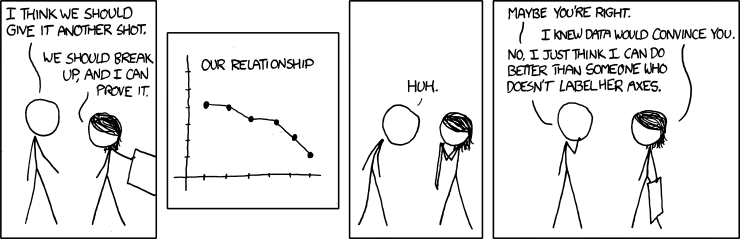
\includegraphics[width=\textwidth]{xkcd_convincing.png}
\end{frame}

\begin{frame}{Use Meaningful Data (XKCD)}
  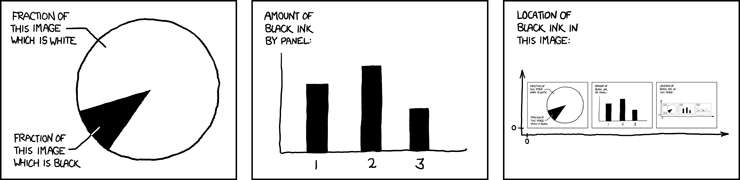
\includegraphics[width=\textwidth]{xkcd_self_description.png}
\end{frame}

\begin{frame}{Use Related Data (XKCD)}
  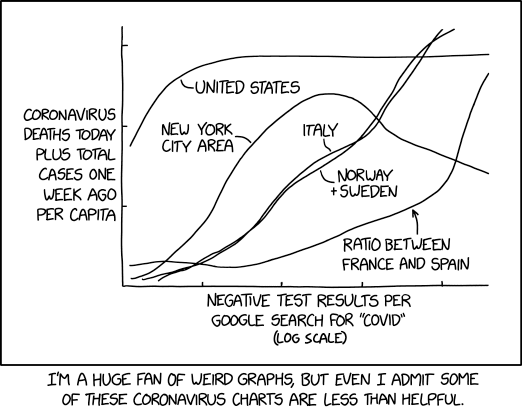
\includegraphics[width=\textwidth]{xkcd_coronavirus_charts.png}
\end{frame}

\begin{frame}{Do Not Mislead (XKCD)}
\centering
  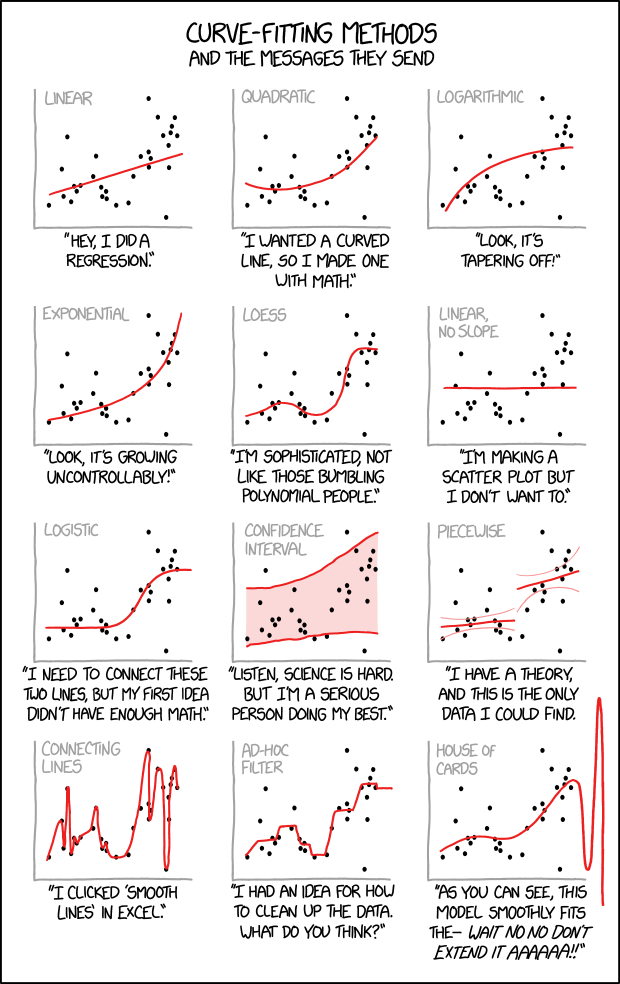
\includegraphics[height=3.5in]{xkcd_curve_fitting.png}
\end{frame}

\begin{frame}{Choose Your Axes Meaningfully}
\centering
  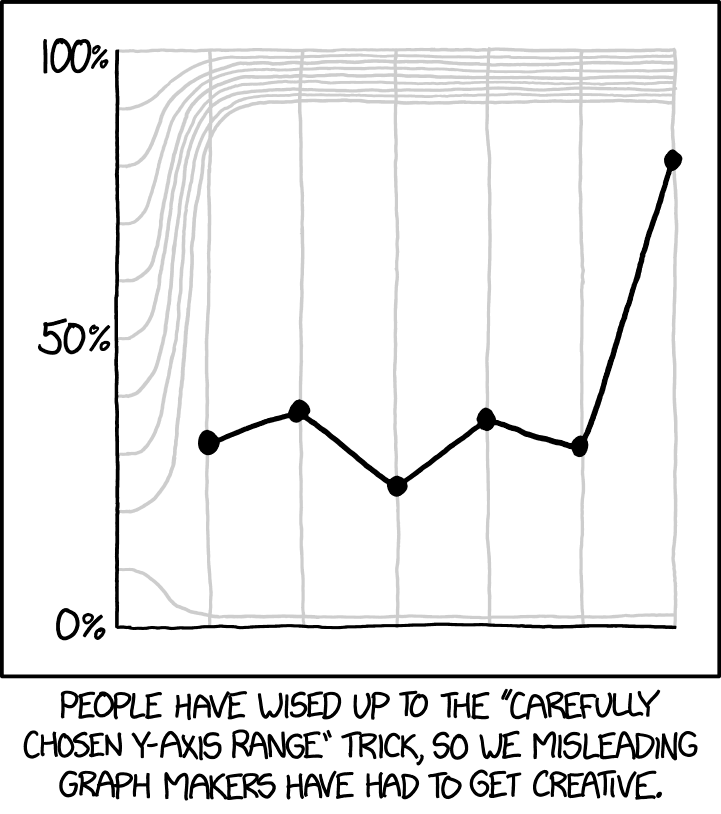
\includegraphics[height=3.2in]{xkcd_y_axis_2x.png}
\end{frame}

\begin{frame}{Be Careful When Extrapolating (XKCD)}
\centering
  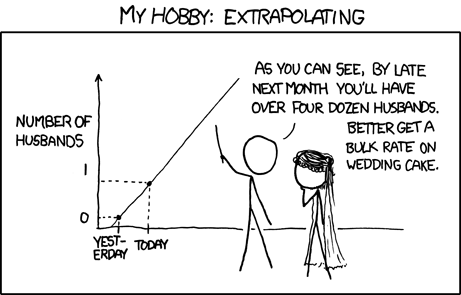
\includegraphics[width=\textwidth]{xkcd_extrapolating.png}
\end{frame}

\begin{frame}{Verify Trends (XKCD)}
\centering
  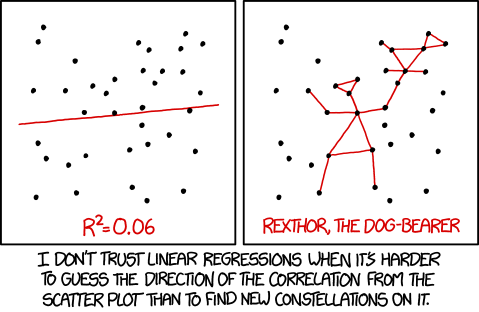
\includegraphics[width=\textwidth]{xkcd_linear_regression.png}
\end{frame}

\begin{frame}{Use Appropriate Scales (XKCD)}
\centering

  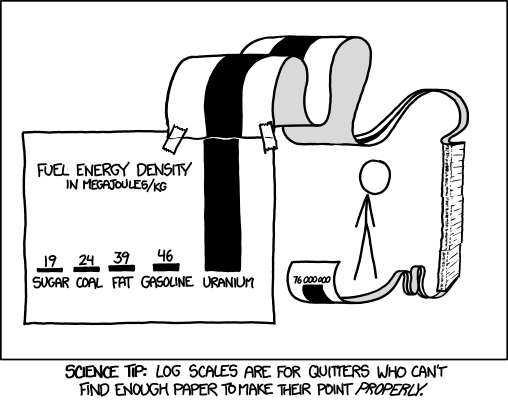
\includegraphics[width=\textwidth]{xkcd_log_scale.png}
\end{frame}

\begin{frame}{Don't Lose Your Point}
\centering
  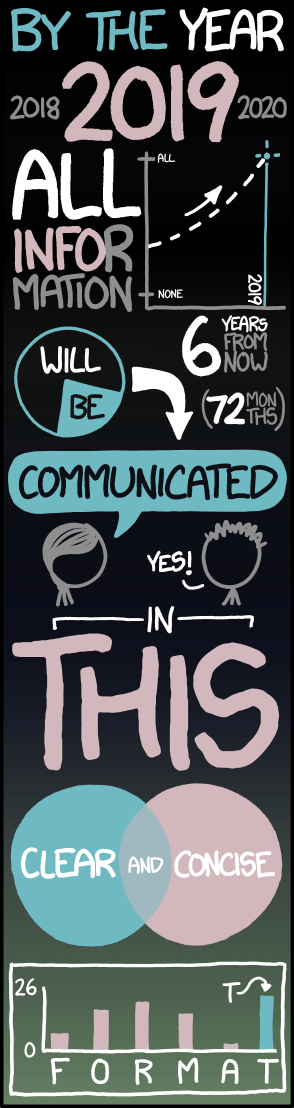
\includegraphics[height=3.3in]{xkcd_tall_infographics.png}
\end{frame}

\begin{frame}{Dark Patterns -- Truncated Axes}
\centering
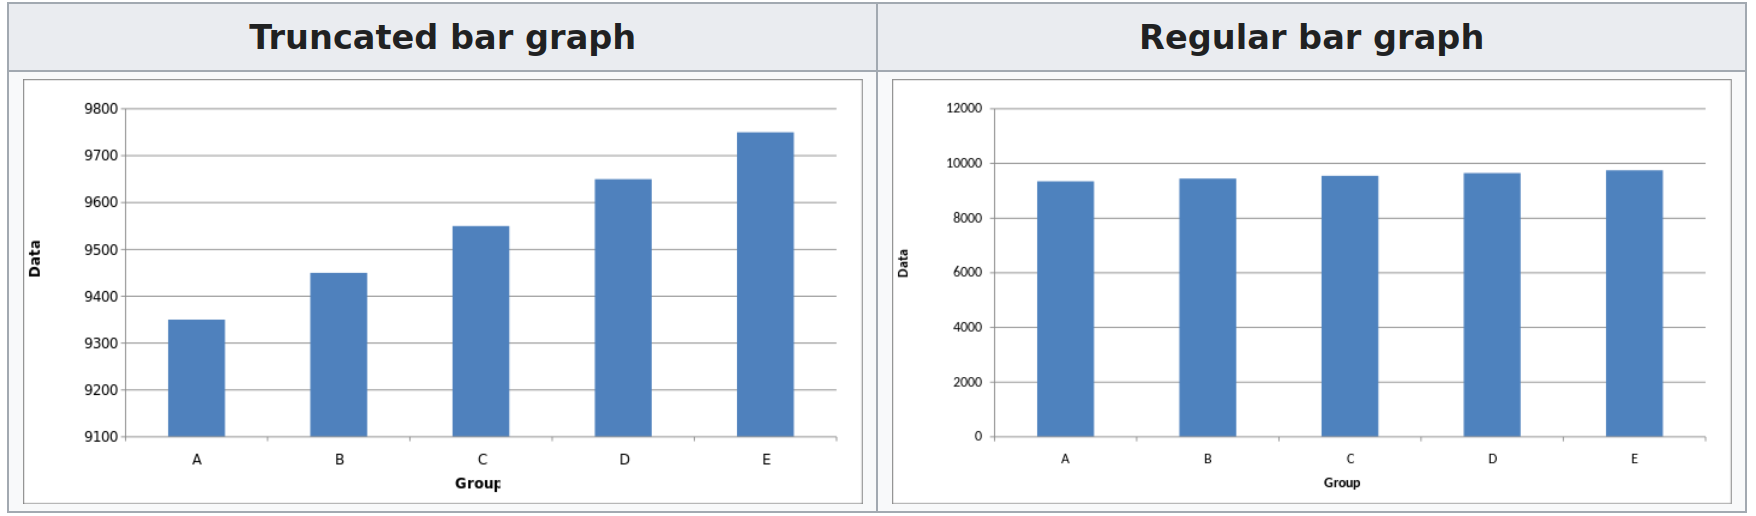
\includegraphics[width=\textwidth]{screen3.png}

\scriptsize\url{https://en.wikipedia.org/wiki/Misleading_graph}
\end{frame}

\begin{frame}{Dark Patterns -- Omitted Data}
\centering
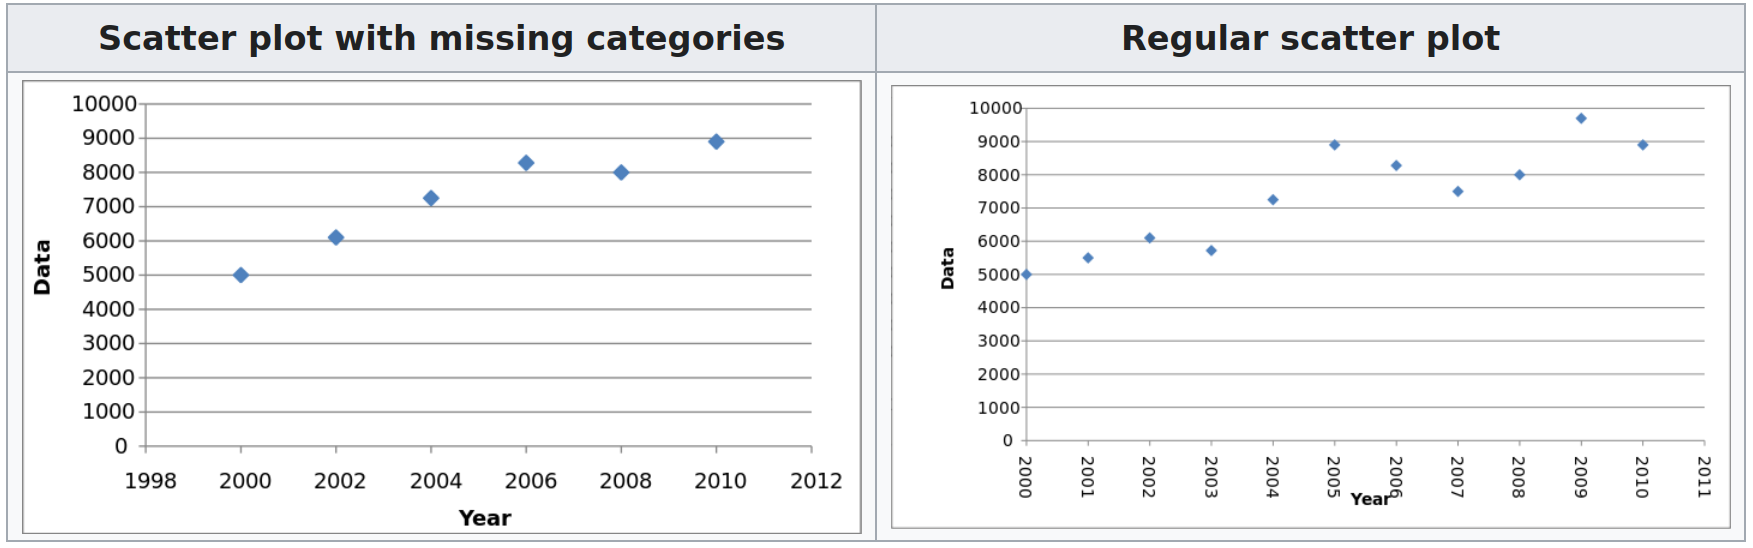
\includegraphics[width=\textwidth]{screen5.png}

\scriptsize\url{https://en.wikipedia.org/wiki/Misleading_graph}
\end{frame}

\begin{frame}{Dark Patterns -- 3D Pie Charts}
\centering
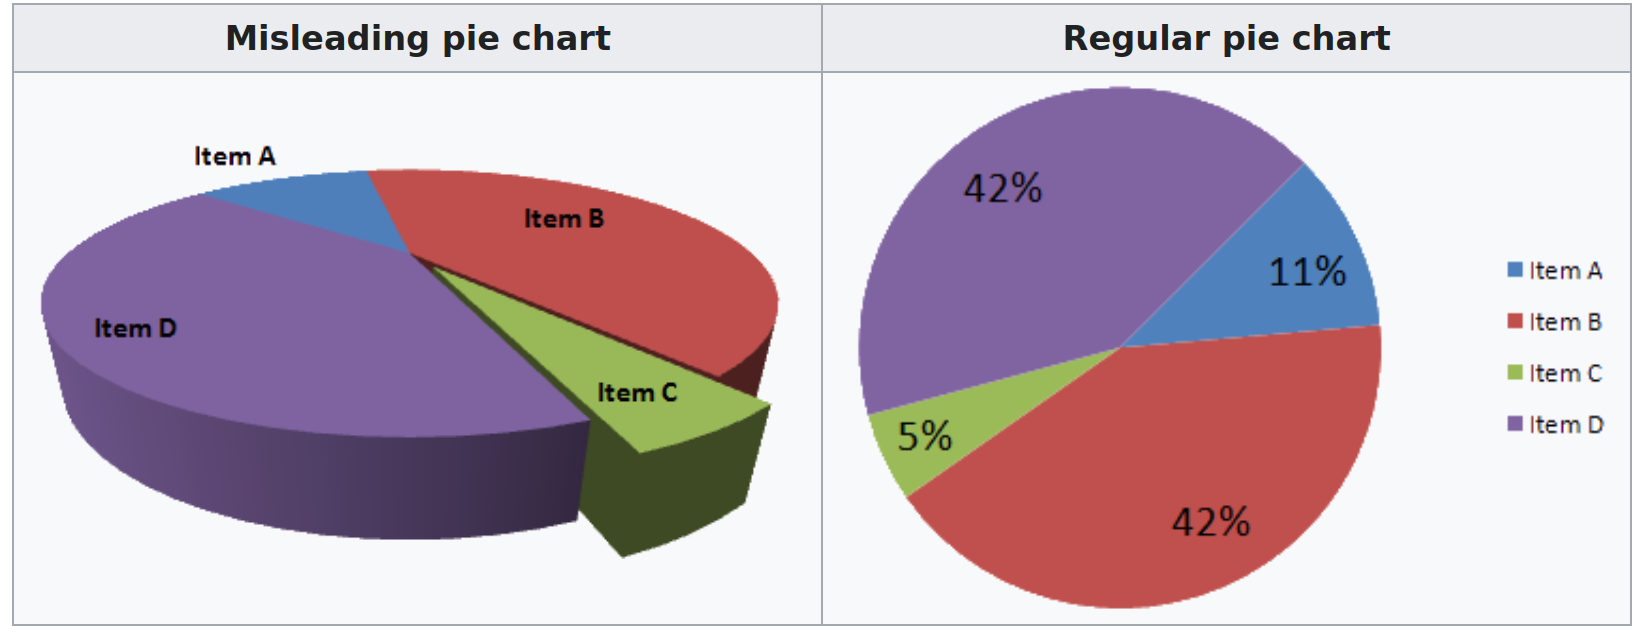
\includegraphics[width=\textwidth]{screen6.png}

\scriptsize\url{https://en.wikipedia.org/wiki/Misleading_graph}
\end{frame}

\begin{frame}{Dark Patterns -- Comparing Pie Charts}
\centering
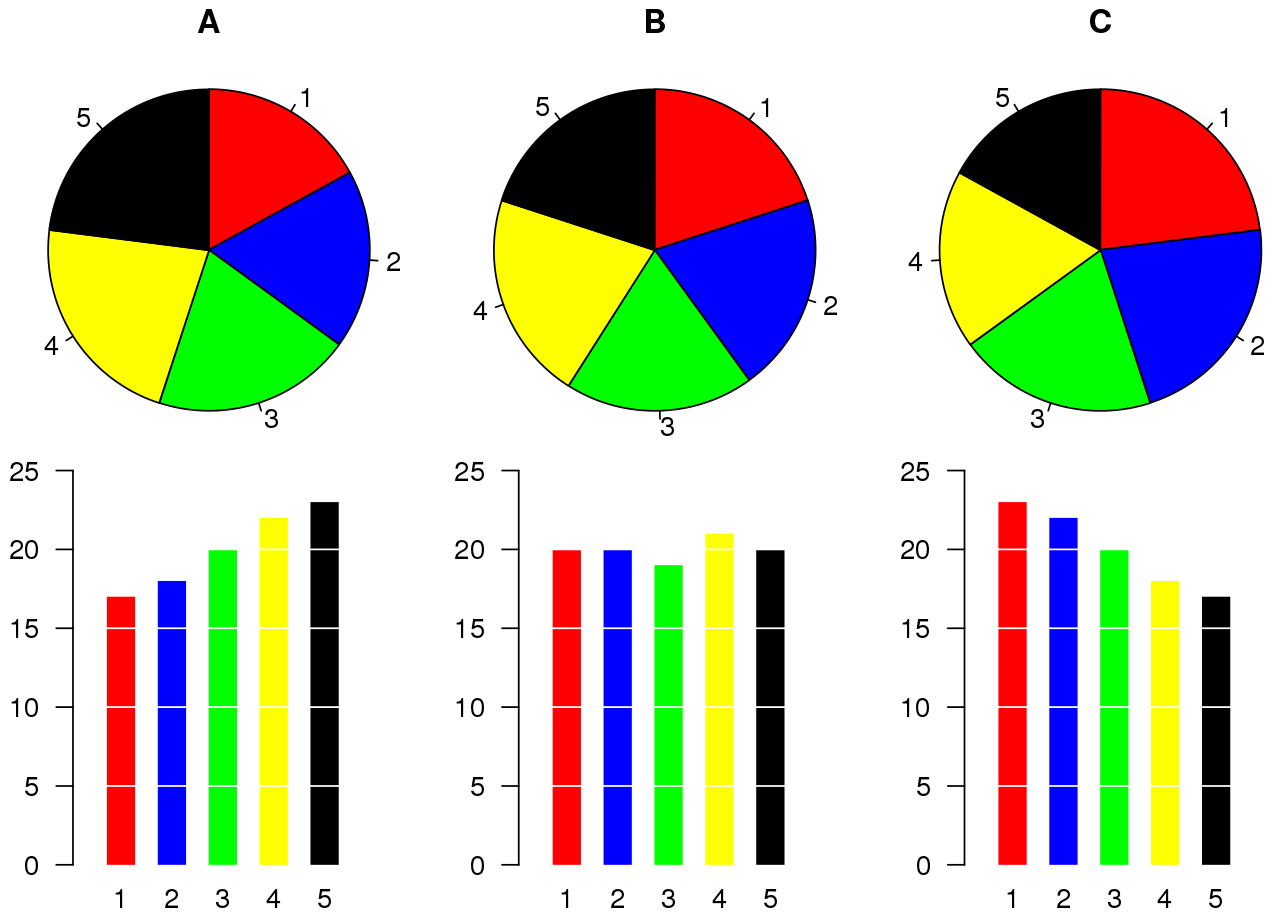
\includegraphics[width=\textwidth]{screen7.png}

\scriptsize\url{https://en.wikipedia.org/wiki/Misleading_graph}
\end{frame}

\begin{frame}{Dark Patterns -- Scaling Axes and Aspect Ratios}
\centering
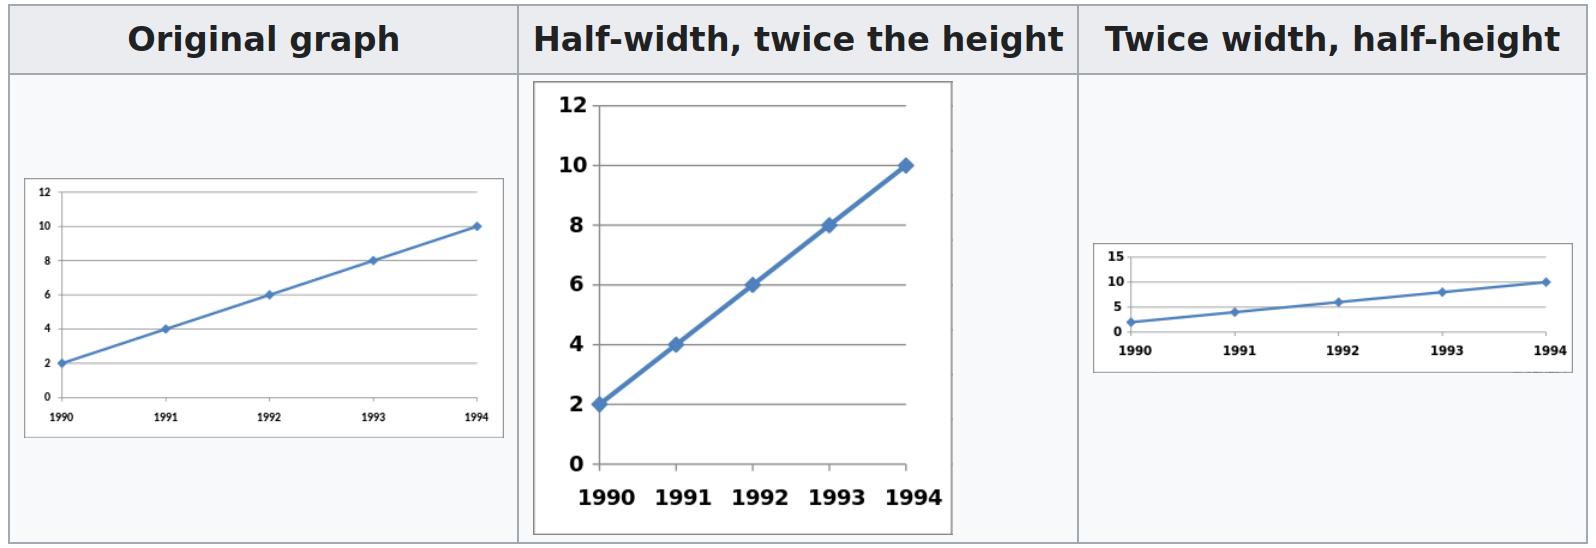
\includegraphics[width=\textwidth]{screen4.png}

\scriptsize\url{https://en.wikipedia.org/wiki/Misleading_graph}
\end{frame}

\begin{frame}{Dark Patterns -- Scaling Multiple Dimensions}
\centering
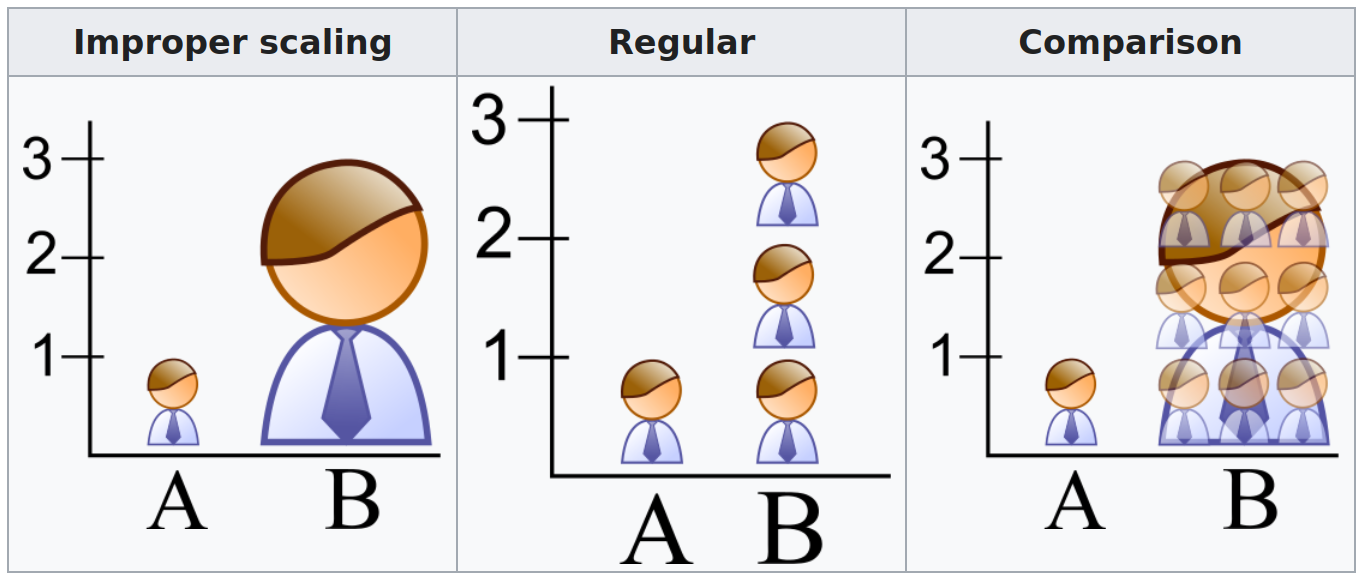
\includegraphics[width=\textwidth]{screen1.png}

\scriptsize\url{https://en.wikipedia.org/wiki/Misleading_graph}
\end{frame}

\begin{frame}{Special Types of Data and Visual Analytics}
	\begin{itemize}
		\item Streaming data
		\begin{itemize}
			\item Continually changing
			\item Limited buffers/windows
		\end{itemize}
		\item Spatial, geographic, map data
		\begin{itemize}
		   \item Geo aware, irregular map boundaries, image overlays
		\end{itemize}
		\item Network data
		\begin{itemize}
		   \item Vertices and vertex types, edges and edge types
		\end{itemize}
		\item Text data
		\begin{itemize}
		   \item Unstructured text, e.g. from social media or web sites
		\end{itemize}
	\end{itemize}
\end{frame}

\begin{frame}{Plot Elements}
	\begin{block}{Map Data to Plot Elements}
	\begin{itemize}
		\item X, Y axis
		\item Colour (point, line, fill)
		\item Transparency (''alpha'')
		\begin{itemize}
		   \item \alert{Be aware of print versus screen or color vision deficiency}
		\end{itemize}
		\item Pattern (fill)
		\item Size, Weight/Width (point, line)
		\item Shape, Style (pint, line)
	\end{itemize}
	\end{block}
	\begin{block}{Other Plot Elements}
		\begin{itemize}
			\item Title, sub-title, captions
			\item Axis titles, axis labels and ''ticks''
			\item Legend(s)
		\end{itemize}
	\end{block}
\end{frame}

\begin{frame}{Colour Palettes}
\begin{block}{Desirable Characteristics}
\begin{itemize} 
  \item Colourful (range of values)
  \item Perceptually uniform (even perceptual distances)
  \item Robust to colourblindness (CVD)
  \item Pretty
\end{itemize}
\end{block}

\begin{block}{Typical of Colour Palettes}
\begin{itemize}
  \item {\bf Monochrome/Sequential}, i.e. light to dark within a single colour
  \item {\bf Divergent}, i.e. from one colour to another via white
  \item {\bf Spectral}, uses a large number of colours
  \item {\bf Bivariate}, e.g. combination or RGB and CMY
\end{itemize}
Colour palettes may be continuous, discrete, or categorical
\end{block}
\end{frame}

\begin{frame}{}
\centering

  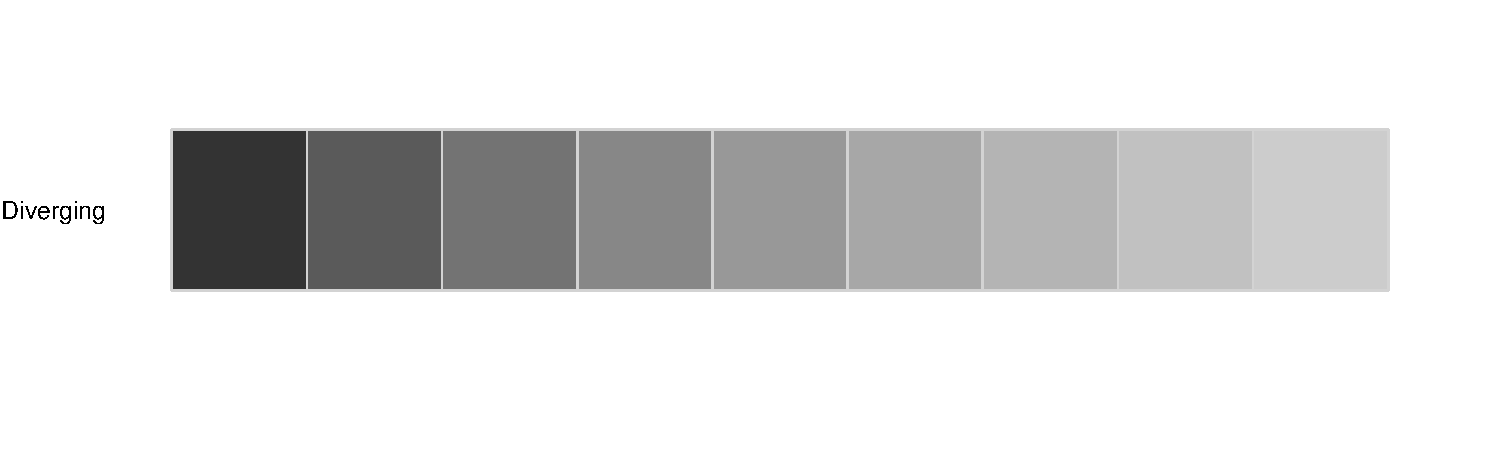
\includegraphics[width=.7\textwidth]{monochromatic.pdf}
  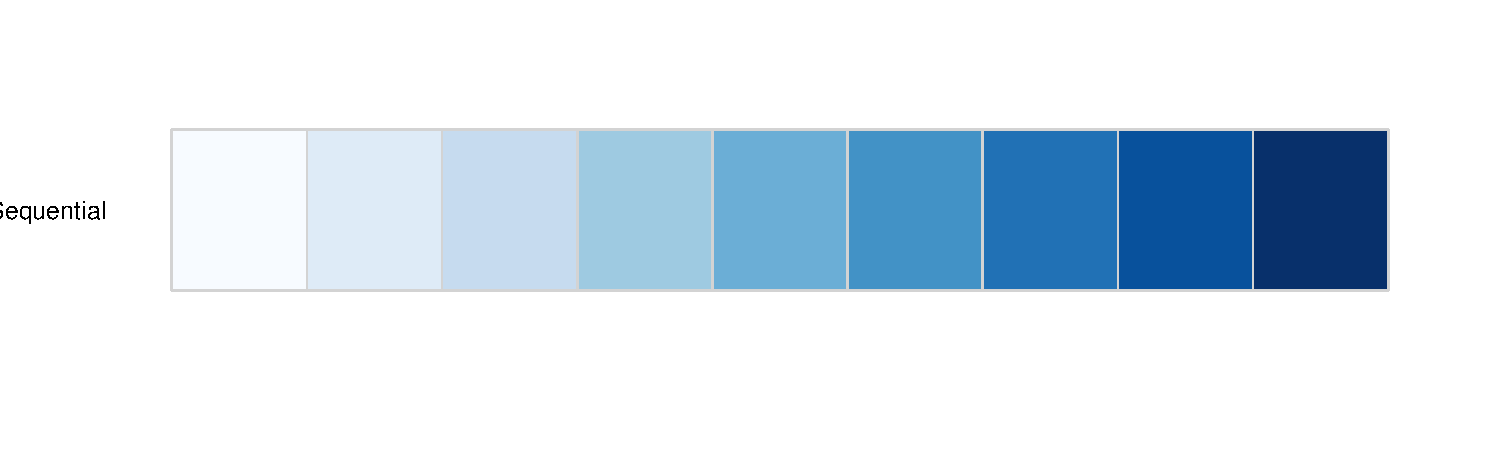
\includegraphics[width=.7\textwidth]{sequential.pdf}
  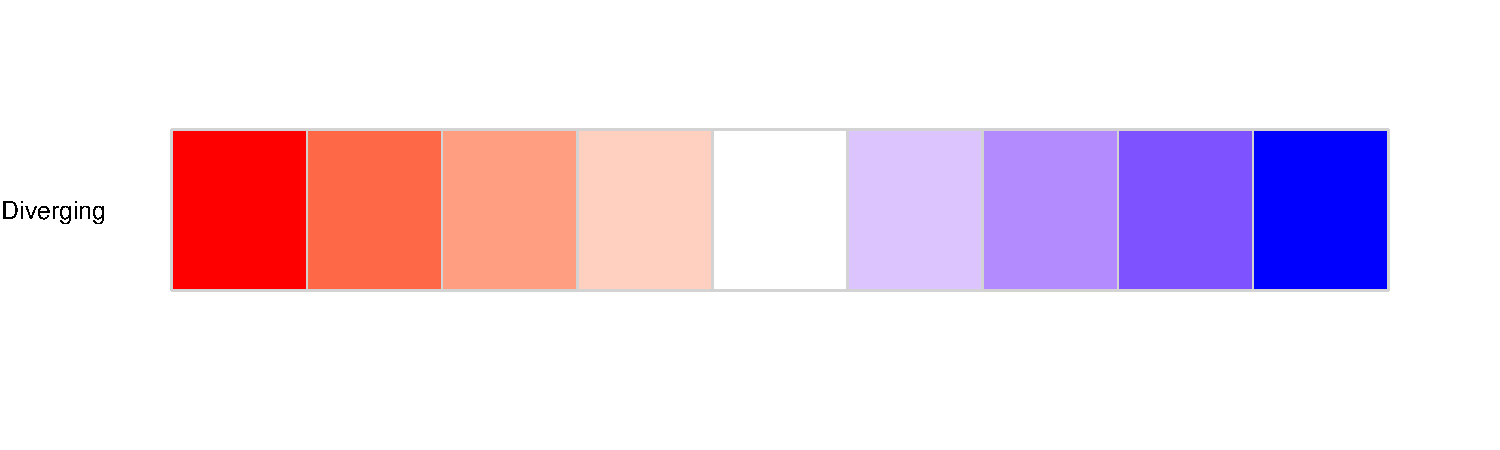
\includegraphics[width=.7\textwidth]{diverging.pdf}
  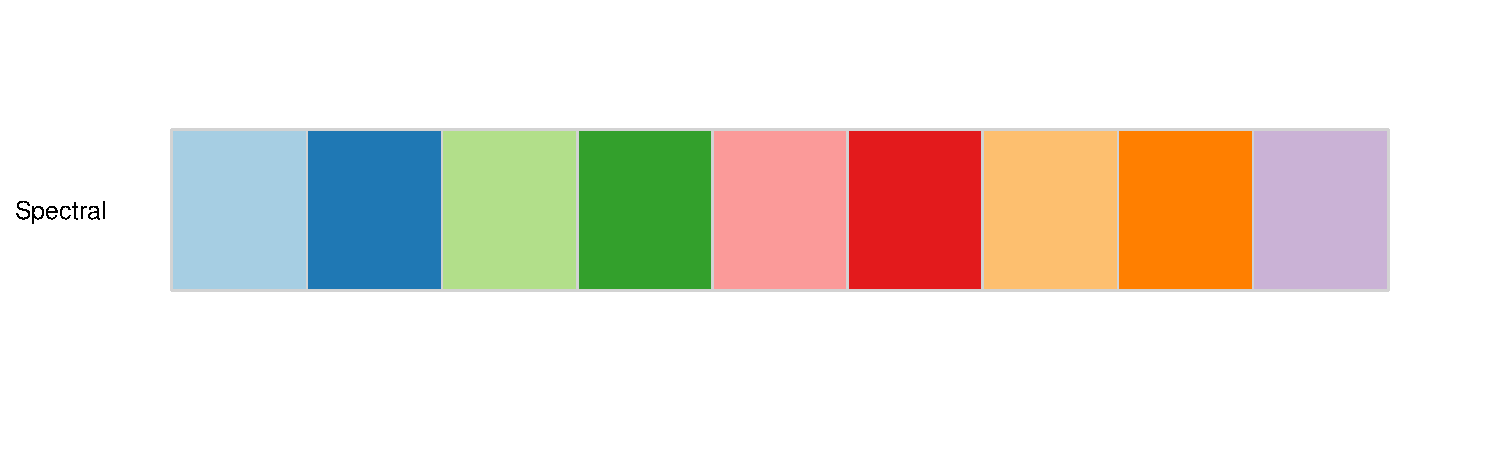
\includegraphics[width=.7\textwidth]{brewer.paired.pdf}
\end{frame}

\begin{frame}{CVD (Colour Vision Deficiency)}
\begin{itemize}
  \item Monochromatism
  \item Protanopia (missing ''S-cone'', blue)
  \item Deuteranopia (missing ''M-cone'', green)
  \item Tritanopia (missing ''L-cone'', red)
\end{itemize}
\vspace{1cm}
\centering
1 in 12 men have CVD \\
1 in 200 women have CVD \\
2.6 million Canadians are colour blind
\end{frame}

\begin{frame}{Original}
  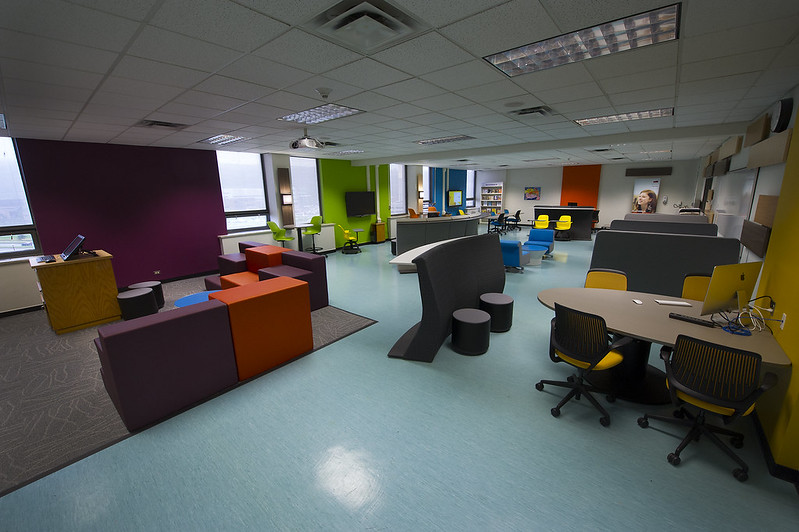
\includegraphics[width=\textwidth]{photo.jpg}
  \centering
  MUN Faculty of Education Class Room \\
  {\tiny Copyright Memorial University of Newfoundland}
\end{frame}

\begin{frame}{Simulated Colour Vision Deficiencies}
\begin{tabular}{cc} 
  \includegraphics[width=.48\textwidth]{desaturate\_photo.jpg} &
  \includegraphics[width=.48\textwidth]{protan\_photo.jpg} \\ 
  Monochromatism & Protanopia \\ 
  \includegraphics[width=.48\textwidth]{deutan\_photo.jpg} &
  \includegraphics[width=.48\textwidth]{tritan\_photo.jpg} \\ 
  Deuteranopia & Tritanopia \\ 
\end{tabular}
\end{frame}
    
\begin{frame}{Example: Colourbrewer Palette ''Paired''}
  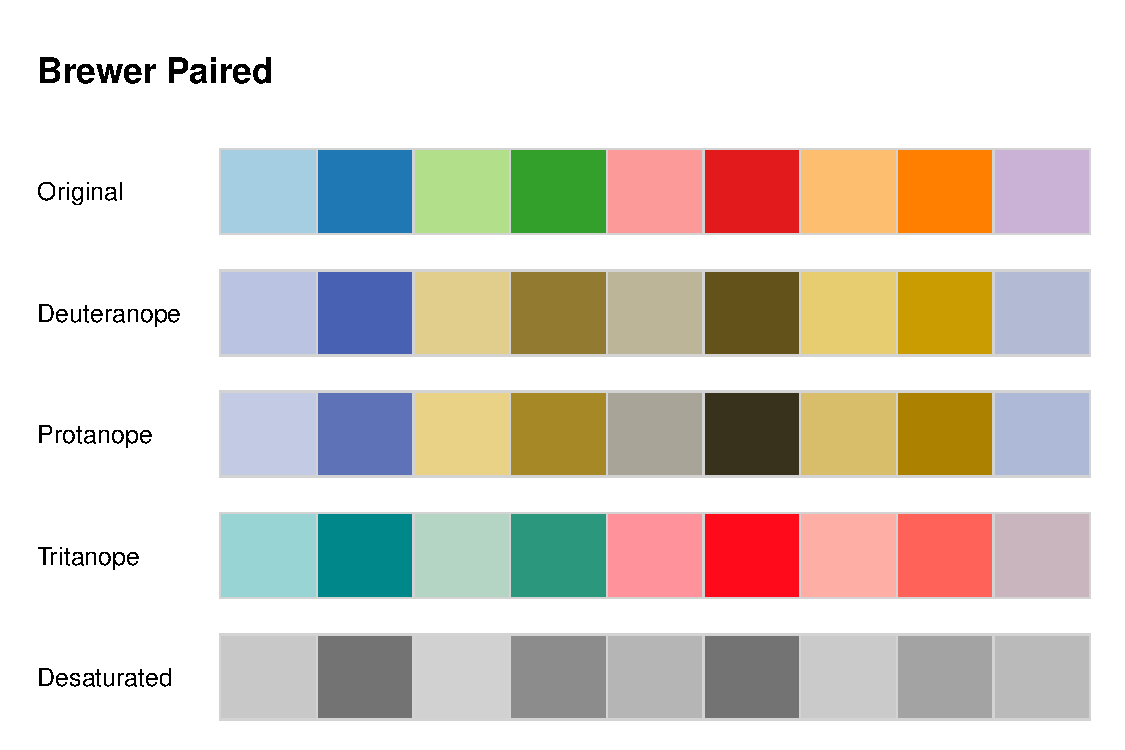
\includegraphics[width=\textwidth]{brewer.paired.cvd.pdf}
\end{frame}

\begin{frame}{Viridis Colour Palette}
  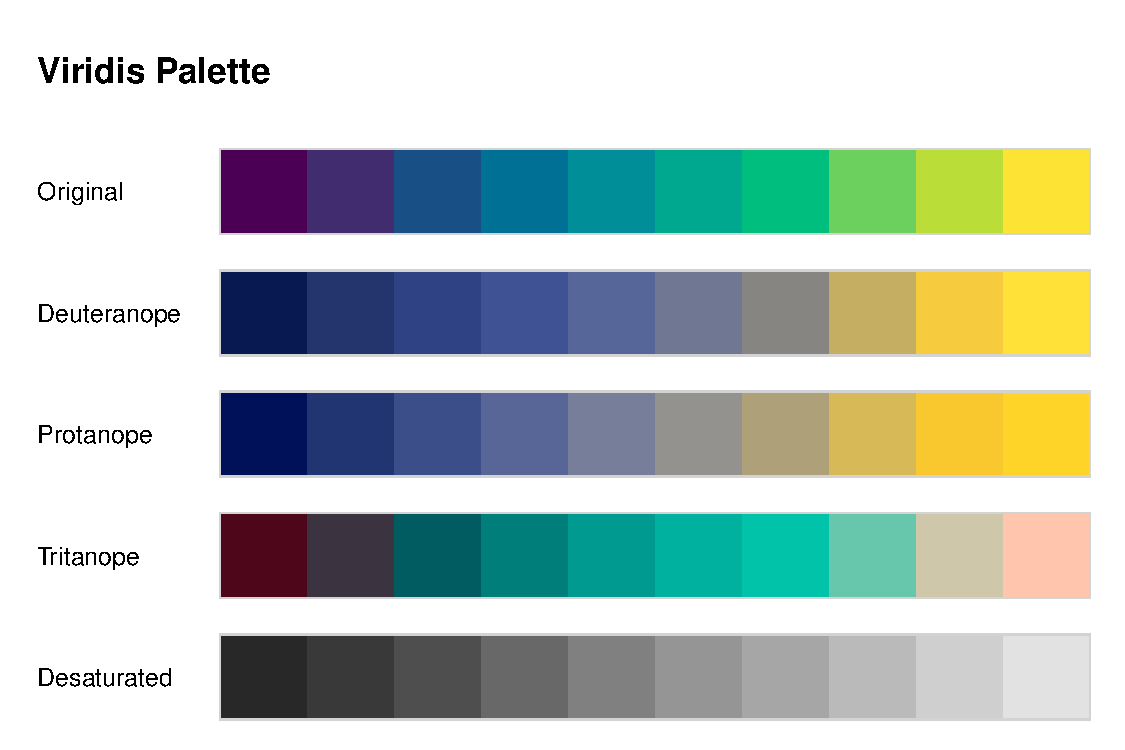
\includegraphics[width=\textwidth]{viridis.plot.pdf}
\end{frame}


\begin{frame}{Plots for One Variable}
\begin{block}{Continuous}
\begin{itemize}
  \item {\bf Area}: Degree of change over time, or relationship of parts to aggregate
  \item {\bf Density, Dot, Frequency, Histogram}: Show frequency distribution of data
\end{itemize}
\end{block}

\begin{block}{Discrete}
\begin{itemize}
  \item {\bf Bar}: Connections among individual things, compare items of different groups
  \item {\bf Pie}: Relationships of parts to aggregate
\end{itemize}
\end{block}
\end{frame}

\begin{frame}{Plots for Two Variables}
\begin{block}{Both Continuous}
\begin{itemize}
  \item {\bf Point}: Connections among numeric values, show multiple groups of data
  \item {\bf Lines, Local Regression}: Relationships/correlations among multiple data series or over time
  \item {\bf Text / Label}: Frequency of labels in content/document
\end{itemize}
\end{block}

\begin{block}{One Discrete, One Continuous}
\begin{itemize}
  \item {\bf Column}: Correlations among things or information changes over time
  \item {\bf Box, Dot, Violin}: Compare distributions between many groups, display spread and skew of data
\end{itemize}
\end{block}
\end{frame}

\begin{frame}{Plots for Two Variables, cont'd}
	\begin{block}{Both Discrete}
		\begin{itemize}
			\item {\bf Points/Counts}: Magnitude of counts
			\item {\bf Jitter}: Plots of data points
		\end{itemize}
	\end{block}
	\begin{block}{Distributions}
		\begin{itemize}
			\item {\bf Bin2D, Density2D, Hex}: Shows frequency of values over two continuous variables
		\end{itemize}
	\end{block}
\end{frame}

\begin{frame}{Plots for Three Variables}
	\begin{block}{Continuous}
		\begin{itemize}
			\item {\bf Contour, Raster and Tile}: Shows relationships among three data series
		\end{itemize}
	\end{block}
\end{frame}

\begin{frame}{Visualizing Errors and Uncertainty}
\begin{block}{Purpose}
	\begin{itemize}
		\item Give a general idea of how precise a value is, or how far a value might be from the true value
		\item Used to augment a given visualization
	\end{itemize}
\end{block}
\begin{block}{Common Visualization Styles}
\begin{itemize}
  \item Crossbar
  \item Errorbar
  \item Range (line, point)
\end{itemize}  
\end{block}
\end{frame}

\begin{frame}{Selected Graphics Libraries and Frameworks}
\begin{block}{R}
\begin{itemize}
  \item GGPlot (and related libraries such as GGPattern)
  \item Plotly for R
  \item GGVis (for Dashboards)
  \item Shiny (for Dashboards)
\end{itemize}
\end{block}
\begin{block}{Python}
\begin{itemize}
  \item Matplotlib
  \item Seaborn
  \item Plotnine (''GGPlot for python'')
  \item Plotly (Express, GO, Dash)
  \item Shiny (for Dashboards)
\end{itemize}
\end{block}
\begin{block}{Web \& JS}
\begin{itemize}
  \item D3, ChartJS, GoogleCharts
\end{itemize}
\end{block}
\end{frame}

\begin{frame}{Example Dataset}
\begin{itemize}
  \item Government of Canada, Open Government Portal
  \item Fuel Consumption Ratings -- Battery-electric vehicles -- 2012--2023
  \item Last updated Oct 10, 2023
  \item \href{https://open.canada.ca/data/en/dataset/98f1a129-f628-4ce4-b24d-6f16bf24dd64}{https://open.canada.ca/data/en/dataset/98f1a129-f628-4ce4-b24d-6f16bf24dd64}
\end{itemize}
\centering
\footnotesize

	\begin{tabular}{|l|l|} \hline
	  {\bf Column} & {\bf Data Type} \\ \hline \hline
	  Make & Discrete \\ 
	  Model & Discrete \\
	  Year & Numeric \\
	  Category & Discrete\footnote{Small, Midsize, Large, Pickup, SUV, Station Wagon, etc.} \\
	  City & Numeric\footnote{Fuel consumption in l/100km equivalent} \\
	  Hwy & Numeric \\
	  Comb & Numeric \\
	  Range & Numeric\footnote{Range in km} \\ \hline
	\end{tabular}
\end{frame}

\begin{frame}[fragile]{Read Data}
\small
\begin{Rcode}
library(tidyverse)

e <- read.csv('fuel.csv')

e$Year <- as.numeric(e$Year)
e$Category <- as.factor(e$Category)
e$Fuel <- as.factor(e$Fuel)
e$City <- as.numeric(e$City)
e$Hwy <- as.numeric(e$Hwy)
e$Comb <- as.numeric(e$Comb)
e$Range <- as.numeric(e$Range)
e$Annual <- as.numeric(e$Annual)

e.clean <- e
\end{Rcode}
\end{frame}

\begin{frame}[fragile]{Load Graphics Libraries}
\small
\begin{Rcode}
library(ggplot2)
library(ggpattern)
library(ggstream)
library(ggsci)
library(scales)
library(ggrepel)
library(ggradar)
\end{Rcode}
\end{frame}

\begin{frame}[fragile]{Histogram}
\small
\begin{Rcode}
e.clean |>
  ggplot(aes(x=Range)) + 
    geom_histogram(bins=50)
    
ggsave("histogram.pdf", 
       height=5, width=7.5, units='in')
\end{Rcode}
\normalsize

\begin{itemize}
  \item Aesthetic \texttt{aes()} determines mapping of data to plot elements
  \item Add plot functions as needed with their own additional aesthetics and options
  \item Save plot in different formats (PDF, PNG, JPEG, \ldots)
\end{itemize}
\end{frame}

\begin{frame}{Histogram}
  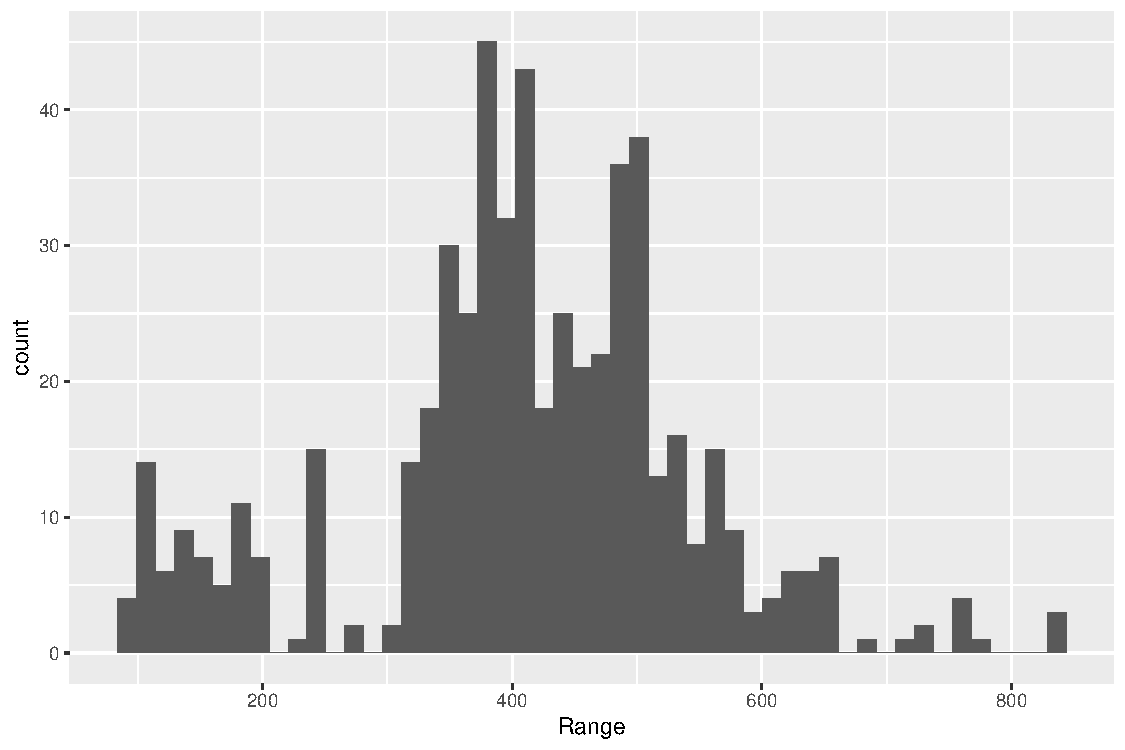
\includegraphics[width=\textwidth]{histogram.pdf}
\end{frame}

\begin{frame}[fragile]{Density Plot}
Prepare some summary statistics:

\small
\begin{Rcode}
mean_v <- e.clean |>
   summarize(mean_v = mean(Range), 
             median_v = median(Range), 
             lower95=quantile(Range, .025), 
             upper95=quantile(Range, .975), 
             maxdensity = max(density(Range)$y))
\end{Rcode}
\end{frame}

\begin{frame}[fragile]{Density Plot \small [cont'd]}
\footnotesize
\begin{Rcode}
e.clean |>
  ggplot(aes(Range)) + 
    geom_density(kernel='gaussian', 
                 fill='lightblue') + 
    labs(x = 'Range (km)', 
         y = 'Proportion of Vehicles', 
         title='Density Plot - Electric Vehicle Range', 
         subtitle='Years 2012 to 2024', 
         caption='Lower and Upper 95 percentile, \
                  median and mean') +
    geom_vline(data=mean_v, 
               aes(xintercept=mean_v), 
               linetype='dashed') +
    geom_vline(data=mean_v, 
               aes(xintercept=median_v), 
               linetype='dotdash') +
    geom_vline(data=mean_v, 
               aes(xintercept=lower95), 
               linetype='dotted') +
\end{Rcode}
\end{frame}

\begin{frame}[fragile]{Density Plot \small [cont'd]}
\footnotesize
\begin{Rcode}
geom_vline(data=mean_v, 
           aes(xintercept=upper95), 
           linetype='dotted') + 
annotate('text', 
   label=paste(' L95=\n ',round(mean_v$lower95),sep=''), 
   x = mean_v$lower95, y = mean_v$maxdensity/2, 
   size=3.5, hjust=0) +
annotate('text', 
   label=paste(' Med=\n ',round(mean_v$median_v),sep=''), 
   x = mean_v$median_v, y = mean_v$maxdensity*3/4, 
   size=3.5, hjust=0) +
annotate('text',
   label=paste(' Mean=\n ',round(mean_v$mean_v),sep=''), 
   x = mean_v$mean_v, y = mean_v$maxdensity*5/8, 
   size=3.5, hjust=0) + 
annotate('text',
   label=paste(' U95=\n ',round(mean_v$upper95),sep=''), 
   x = mean_v$upper95, y = mean_v$maxdensity/2, 
   size=3.5, hjust=0)
\end{Rcode}
\end{frame}

\begin{frame}{Density Plot [cont'd]}
  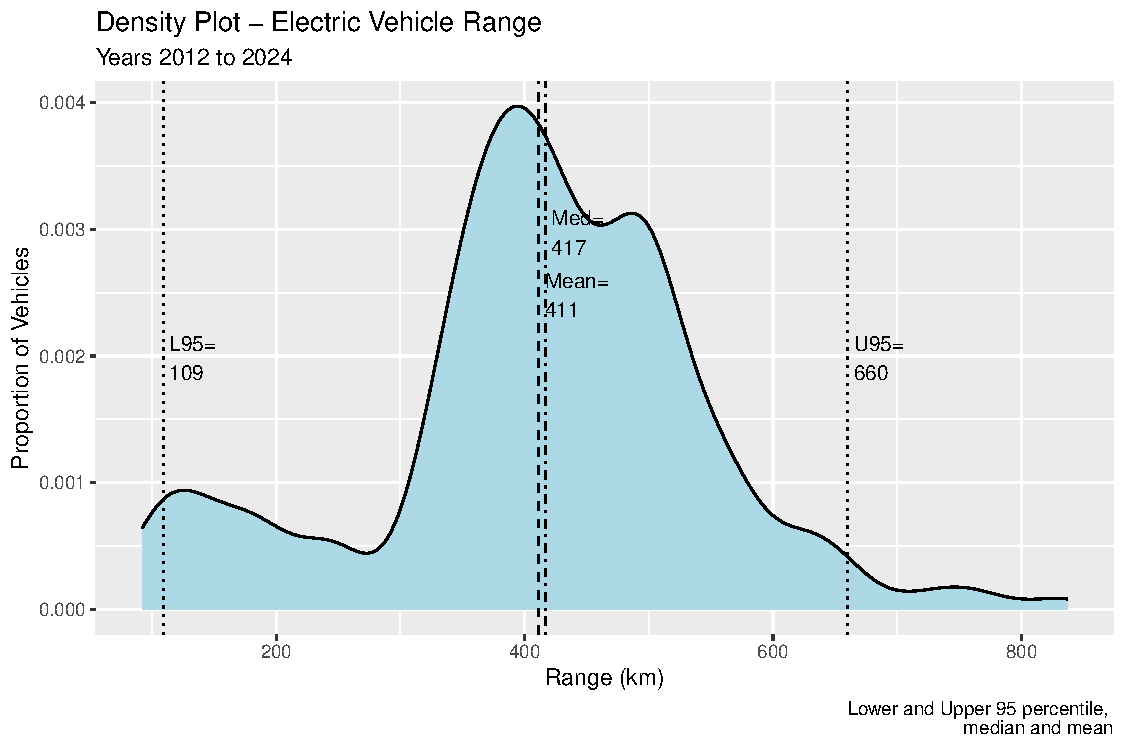
\includegraphics[width=\textwidth]{fuel.density.pdf}
\end{frame}

\begin{frame}{Density Plot [cont'd]}
\begin{itemize}
   \item Add additional elements to a plot with ''\texttt{+}''
   \item Explicitly label plot and axes
   \item \texttt{geom\_vline} and \texttt{annotate} are elements like \texttt{geom\_density} and \texttt{geom\_history} that can be added to plots
   \item \texttt{geom\_vline} does not get its data from the pipe, but from the \texttt{mean\_v} data frame
   \item Annotations can be freely placed in the plot in coordinate system determined by plot axes
\end{itemize}
\end{frame}

\begin{frame}[fragile]{Histogram}
\footnotesize
\begin{Rcode}
...
geom_histogram(aes(y=..density..), bins=50, 
     alpha=0.5, fill='white', color='black', ) +
geom_density(kernel='gaussian', 
     alpha=0.25, fill='lightblue') + 
...
\end{Rcode}
\begin{center}
  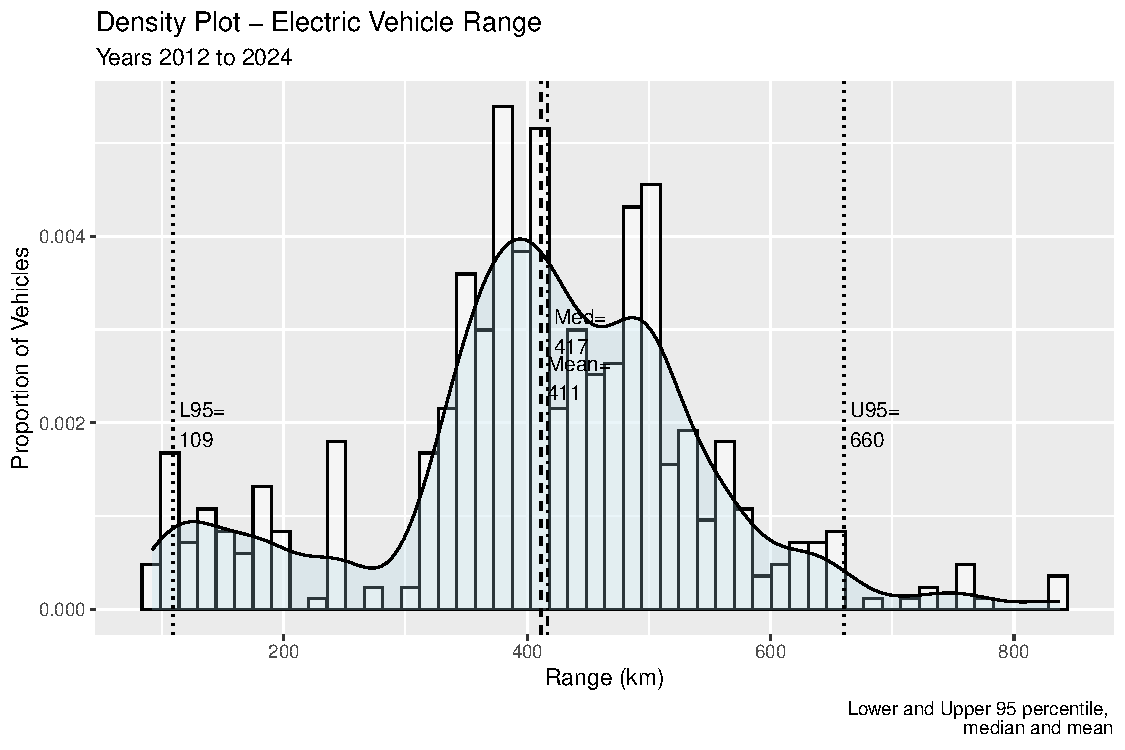
\includegraphics[width=.75\textwidth]{fuel.histogram.pdf}
\end{center}
\end{frame}

\begin{frame}[fragile]{Area Plot}
\footnotesize
\begin{Rcode}
e.clean %>%
  group_by(Year) %>%
  summarize(meanRange = mean(Range)) %>%
  ungroup() %>%
  ggplot(aes(Year, meanRange)) + 
    geom_area(fill='purple') +
    geom_text(aes(label=round(meanRange)), 
              size=5, position='jitter') +
    labs(x='Year', y='Mean Range (km)', 
         title='Vehicle Range by Year', 
         subtitle='Years 2012-2024')
\end{Rcode}
\end{frame}

\begin{frame}{Area Plot}
  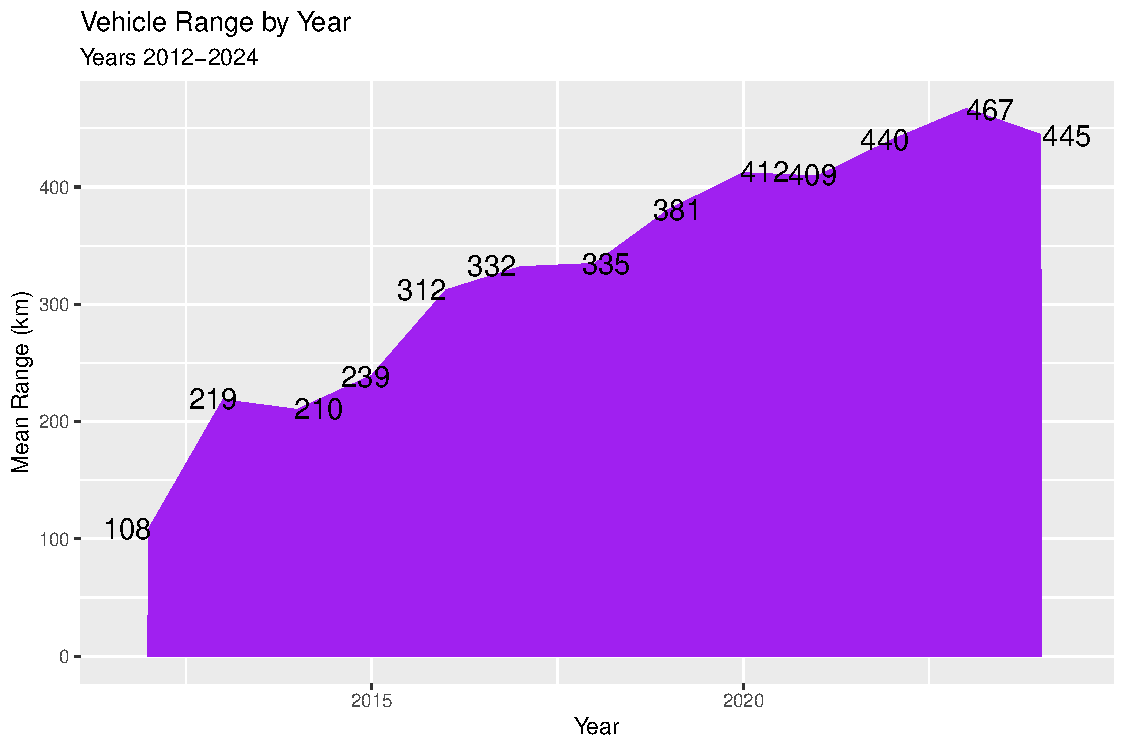
\includegraphics[width=\textwidth]{fuel.areaOneSeries.pdf}
\end{frame}

\begin{frame}[fragile]{Column Chart}
\scriptsize
\begin{Rcode}
e.clean %>%
   group_by(Year) %>%
   summarize(meanCity = mean(City), meanHwy = mean(Hwy)) %>%
   ungroup() %>%
   pivot_longer(cols=c('meanCity', 'meanHwy'), 
                names_to='metric', 
                values_to='consumption') |>
   ggplot(aes(Year, consumption, fill=metric)) +
      geom_col(position='dodge') +
      scale_fill_brewer(palette="Paired") +
      scale_fill_discrete(labels=c("City", "Highway")) + 
      labs(x = 'Year', 
           y='Mean Fuel Consumption\n(l/100km equivalent)', 
           fill='', 
           title='Electric Vehicle Range', 
           subtitle='Years 2012 to 2024')
\end{Rcode}
\end{frame}

\begin{frame}{Column Chart}
  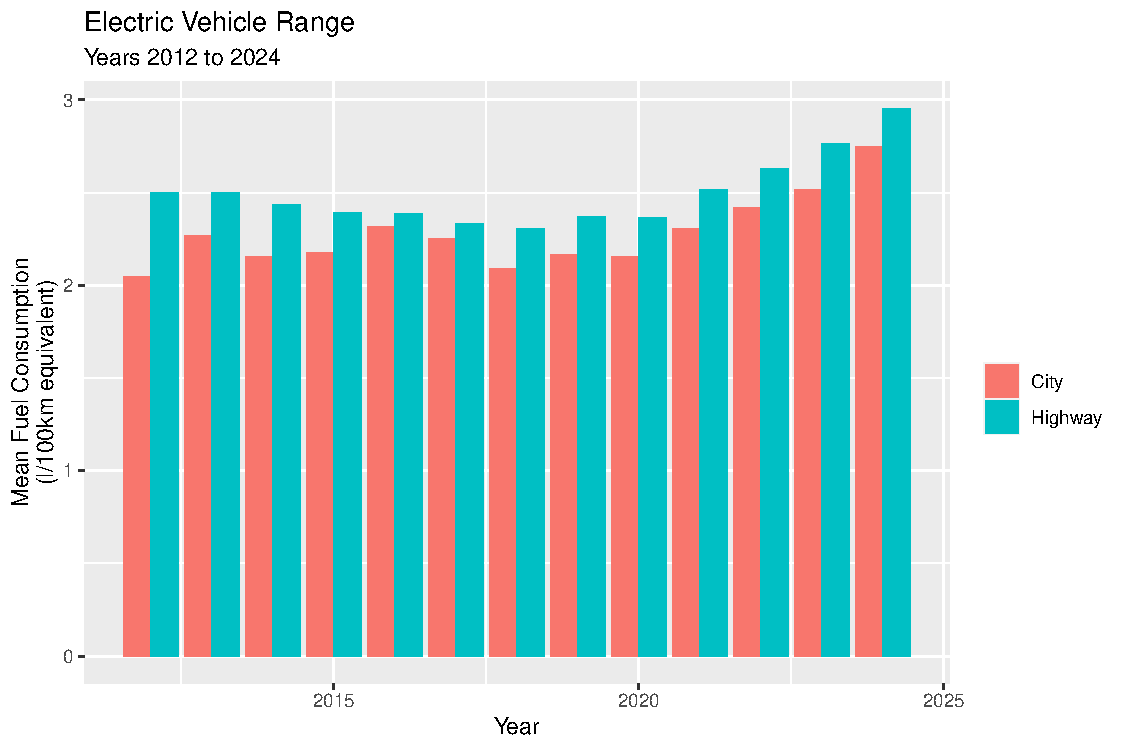
\includegraphics[width=\textwidth]{fuel.columns.pdf}
\end{frame}


\begin{frame}[fragile]{Column Chart (with Patterns)}
Prepare data
\footnotesize
\begin{Rcode}
e.clean %>% 
   group_by(Year) %>%
   summarize(meanCity = mean(City), 
             meanHwy = mean(Hwy)) %>%
   ungroup() %>%
   pivot_longer(
        cols=c('meanCity', 'meanHwy'), 
        names_to='metric', 
        values_to='consumption') %>%
\end{Rcode}
\end{frame}

\begin{frame}[fragile]{Column Chart (with Patterns) \small [cont'd]}
Continued from previous slide ...
\scriptsize
\begin{Rcode}
ggplot(aes(Year, consumption)) +
  geom_col_pattern(
         aes(pattern_type=metric, pattern_angle=metric),
     pattern='polygon_tiling',
     pattern_fill='white', 
     pattern_scale=0.5,
     position='dodge',
     pattern_key_scale_factor=0.4) +
  scale_pattern_type_manual(
     values = c('hexagonal', 'rhombille', 'pythagorean', 
                'truncated_square', 'rhombitrihexagonal', 
                'truncated_trihexagonal'), 
     labels=c("City", "Highway")) + 
  labs(x = 'Year', y='Mean Fuel Consumption', 
       pattern_type='', 
       title='Electric Vehicle Range', 
       subtitle='Years 2012 to 2024') +
  guides(pattern_angle=FALSE, 
         pattern_type=guide_legend(nrow=1)) + 
  theme(legend.key.size=unit(1.5, 'cm'), 
		legend.position='bottom')
\end{Rcode}
\end{frame}


\begin{frame}{Column Chart (with Patterns)}
  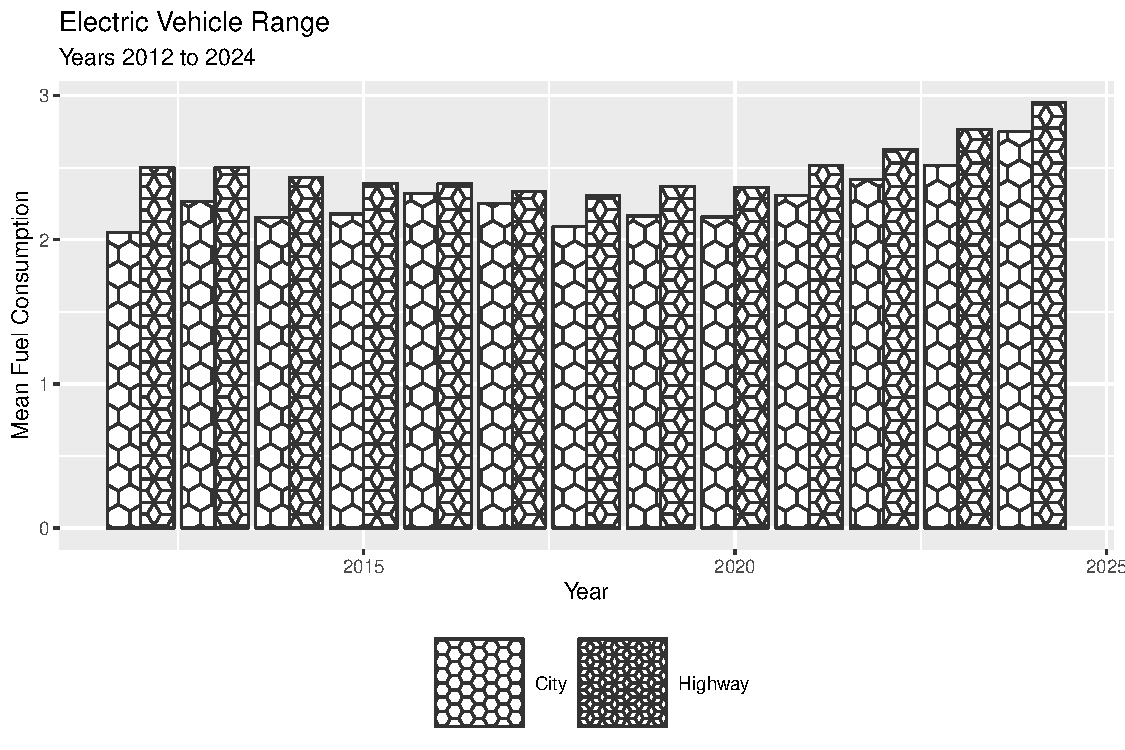
\includegraphics[width=\textwidth]{fuel.columnsPatterns.pdf}
\end{frame}

\begin{frame}[fragile]{Box Plot}
\footnotesize
\begin{Rcode}
e.clean %>% 
  pivot_longer(cols=c('City', 'Hwy'), 
               names_to='metric', 
               values_to='consumption') %>%
ggplot(aes(x=as.factor(Year), 
           y=consumption, 
           fill=metric)) +
  geom_boxplot() +
\end{Rcode}
\end{frame}

\begin{frame}[fragile]{Box Plot}
\footnotesize
\begin{Rcode}
  stat_summary(
    aes(label = round(stat(y), 1)),
    geom = "text", 
    size=2,
    fun.y = function(y) {
	          o<-boxplot.stats(y)$out; 
              if(length(o)==0) NA else o}) + 
  scale_fill_brewer(palette="Paired") +
  labs(x = 'Year', 
    y='Mean Fuel Consumption\n(l/100km equivalent)', 
    fill='', 
    title='Electric Vehicle Range', 
    subtitle='Years 2012 to 2024') +
  theme(legend.key.size=unit(1, 'cm'), 
        legend.position='top')
\end{Rcode}
\end{frame}

\begin{frame}{Box Plot}
  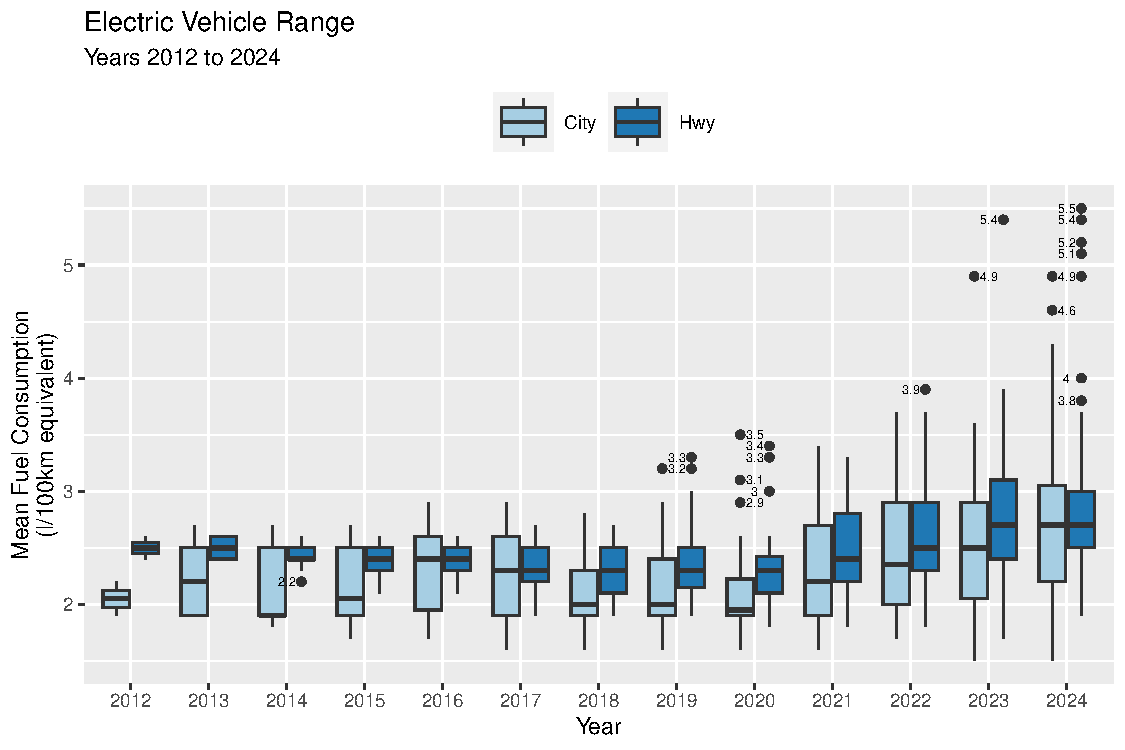
\includegraphics[width=\textwidth]{fuel.box.pdf}
\end{frame}


\begin{frame}{Boxplot (XKCD)}
 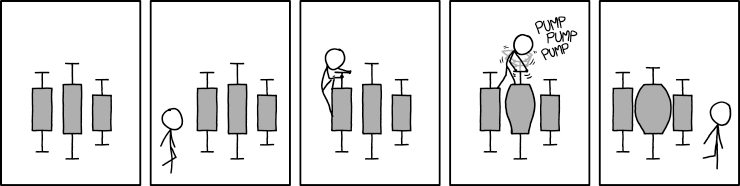
\includegraphics[width=\textwidth]{xkcd_box_plot.png}
\end{frame}

\begin{frame}[fragile]{Violin Plot}
\footnotesize
\begin{Rcode}
e.clean %>% 
  ggplot(aes(x=as.factor(Year), y=Comb)) +
    geom_violin(fill='lightblue') +
    geom_jitter(width=0.15, color='black', 
                size=1, fill=NA, alpha=0.5) + 
    scale_fill_brewer(palette="Paired") +
    labs(x = 'Year', 
         y='Mean Fuel Consumption\n(l/100km equivalent)', 
         fill='', 
         title='Electric Vehicle Range', 
         subtitle='Years 2012 to 2024')
\end{Rcode}
\end{frame}

\begin{frame}{Violin Plot}
  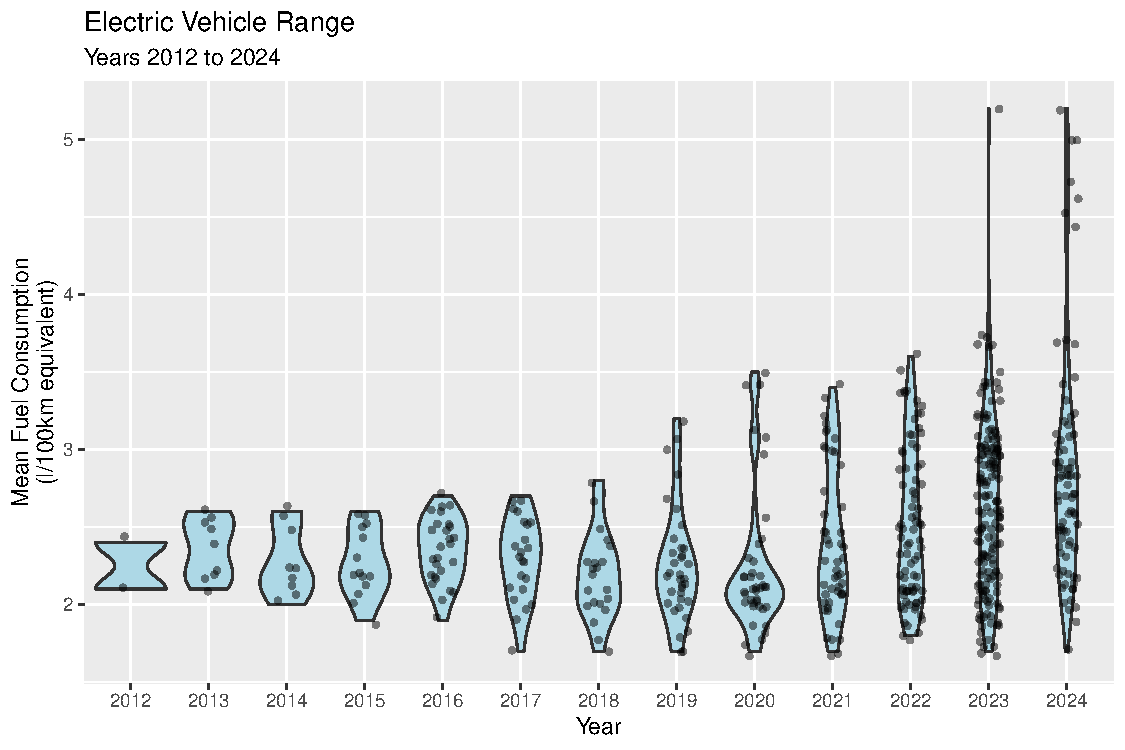
\includegraphics[width=\textwidth]{fuel.violin.pdf}
\end{frame}

\begin{frame}[fragile]{Dot Plot}
\footnotesize
\begin{Rcode}
e.clean %>% 
  ggplot(aes(x=as.factor(Year), y=Comb)) +
    geom_dotplot(binaxis='y', 
                 stackdir='center', 
                 stackratio=0.5,
                 binpositions='all',
                 dotsize=0.5, 
                 color='black', 
                 fill='orange') +
    scale_fill_brewer(palette="Paired") +
    labs(x = 'Year', 
         y='Mean Fuel Consumption\n(l/100km equiv)', 
         fill='', 
         title='Electric Vehicle Range', 
         subtitle='Years 2012 to 2024')
\end{Rcode}
\end{frame}

\begin{frame}{Dot Plot}
  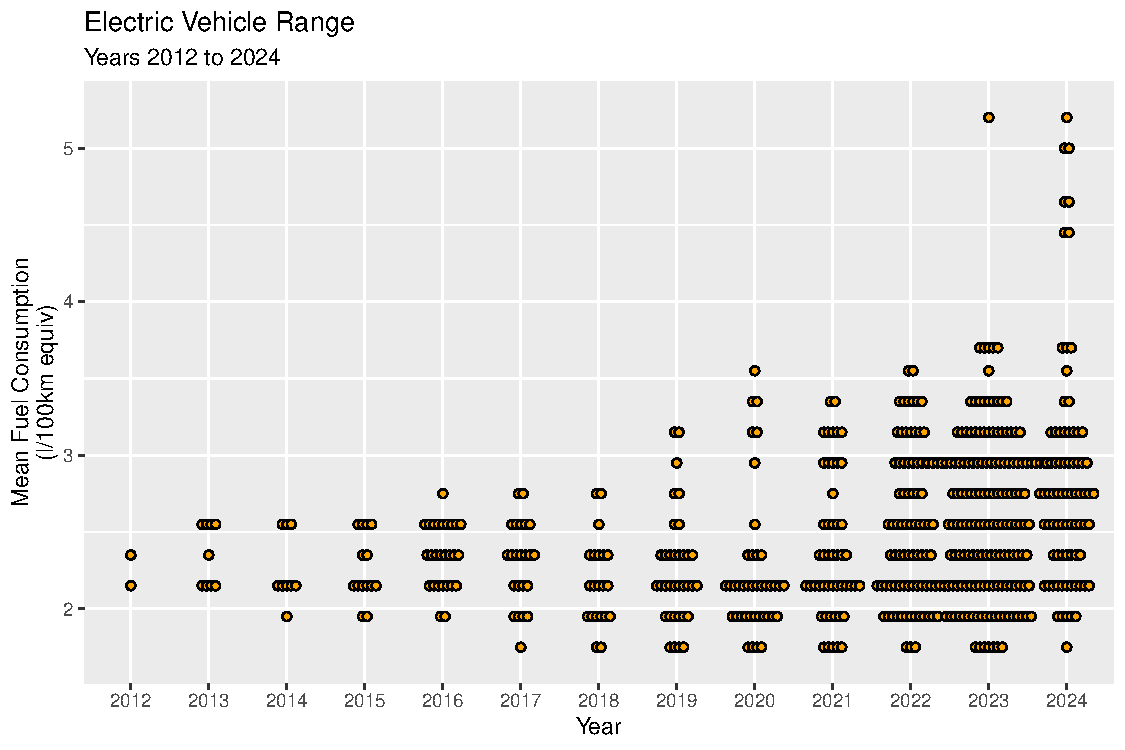
\includegraphics[width=\textwidth]{fuel.dotplot.pdf}
\end{frame}

\begin{frame}[fragile]{Dot Plot (with Violin and Range Summary)}
\footnotesize
\begin{Rcode}
e.clean %>% 
  filter(Year > 2019) %>%
  ggplot(aes(x=as.factor(Year), y=Comb)) +
    geom_dotplot(binaxis='y', 
                 stackdir='center', stackratio=0.5,
                 binpositions='all', dotsize=0.5, 
                 color='black', fill='orange') +
    geom_violin(color='black', fill=NA) + 
    stat_summary(fun.data=mean_sdl, 
                 fun.args=list(mult=1), 
                 size=1, color='blue', 
                 geom="pointrange") +
    scale_fill_brewer(palette="Paired") +
    labs(x = 'Year', 
         y='Mean Fuel Consumption\n(l/100km equiv)', 
         fill='', 
         title='Electric Vehicle Range', 
         subtitle='Years 2020 to 2024') +
     theme(legend.position='none')
\end{Rcode}
\end{frame}

\begin{frame}{Dot Plot (with Violin and Range Summary)}
  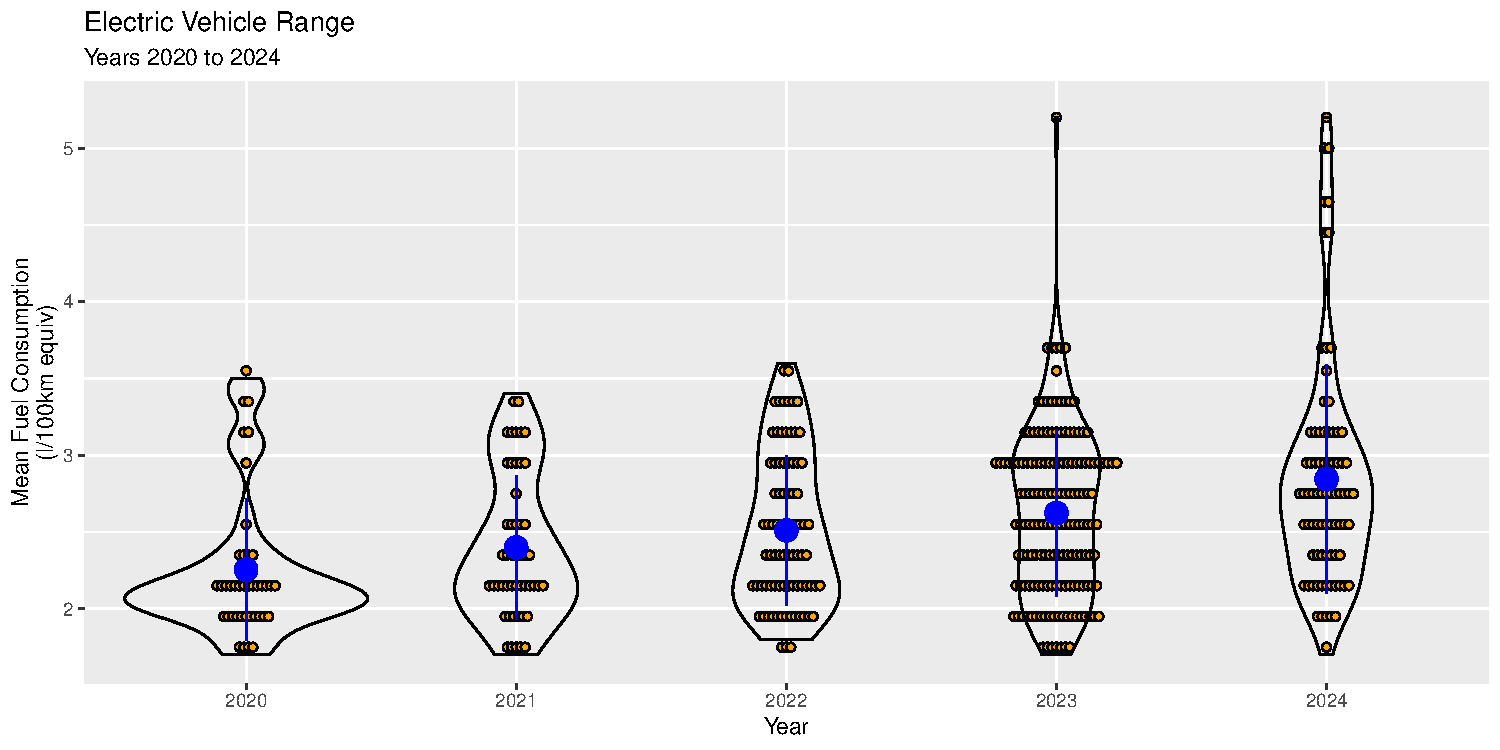
\includegraphics[width=\textwidth]{fuel.dotplotjviolinsummary.pdf}
\end{frame}

\begin{frame}[fragile]{Count Plot}
\scriptsize
\begin{Rcode}
e.clean %>% 
  ggplot(aes(as.factor(Year), as.factor(Category))) +
    geom_count(color='darkolivegreen4')+
    scale_size_area(max_size=10, n.breaks=6) + 
    scale_color_brewer(palette="Paired") +
    scale_y_discrete(
      labels=c('Compact', 'Large', 'Mid-Size', 'Pickup truck', 
               'Subcompact', 'Two-seater', 'SUV (standard)', 
               'SUV (small)', 'Station Wagon (small)')) + 
    guides(color=FALSE) +
    labs(x = 'Year',
         y='Category', 
         fill='', 
         title='Electric Vehicle Models by Category', 
         subtitle='Years 2012 to 2024') +
    theme(legend.background=element_blank(), 
          legend.box.background=element_rect(color='black', 
                                             fill=NA),
          legend.key.size=unit(1, 'cm'))
\end{Rcode}
\end{frame}

\begin{frame}{Count Plot}
  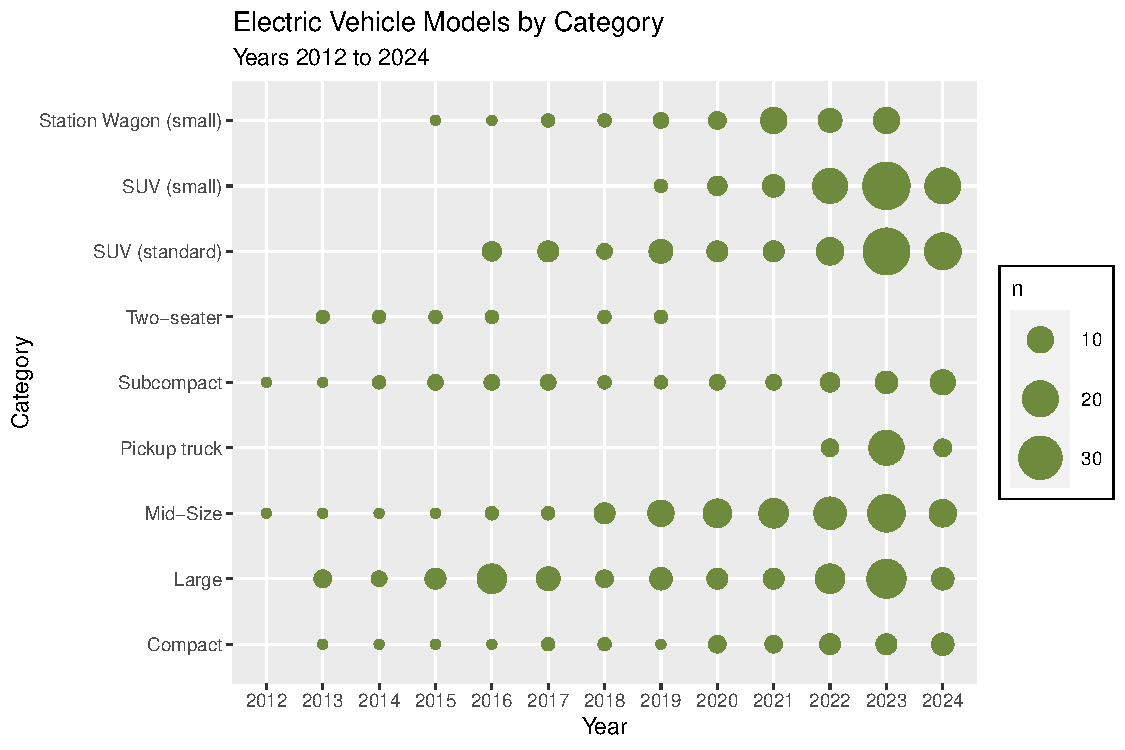
\includegraphics[width=\textwidth]{fuel.count.pdf}
\end{frame}

\begin{frame}[fragile]{Jitter Plot}
\footnotesize
\begin{Rcode}
e.clean %>% 
  ggplot(aes(x=as.factor(Year), 
             y=as.factor(Category), 
             color=as.factor(Year))) +
    geom_jitter(width=0.2, height=0.2) +
    scale_color_manual(values=c25) +
    scale_y_discrete(
      labels=c('Compact', 'Large', 'Mid-Size', 
               'Pickup truck', 'Subcompact',
               'Two-seater', 'SUV (std)', 
               'SUV (sm)', 'Station Wagon (sm)')) + 
    guides(color=FALSE) +
    labs(x = 'Year', 
         y='Category', 
         fill='Make', 
         title='Electric Vehicle Models by Category', 
         subtitle='Years 2012 to 2024')
\end{Rcode}
\end{frame}

\begin{frame}{Jitter Plot}
  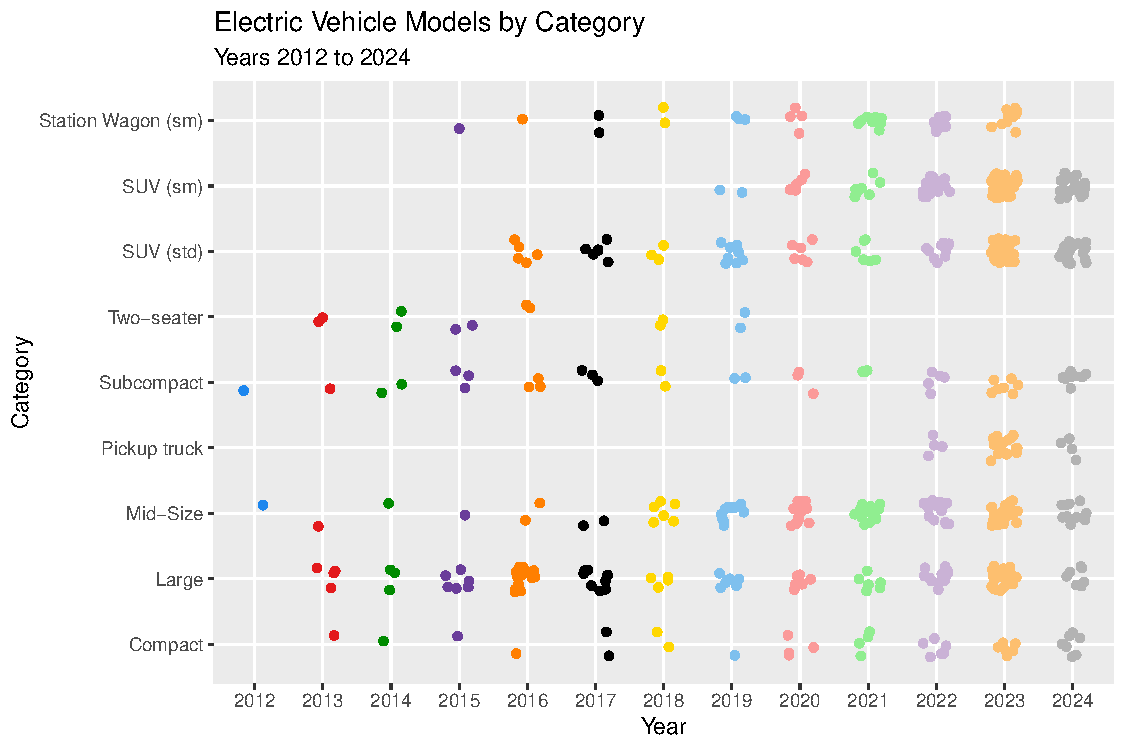
\includegraphics[width=\textwidth]{fuel.jitterdiscrete.pdf}
\end{frame}

\begin{frame}[fragile]{Points Plot}
\footnotesize
\begin{Rcode}
e.clean %>% 
  group_by(Year, Category) %>%
  summarize(totalcount=n(), meanRange=mean(Range)) %>%
  ungroup () %>%
ggplot(aes(x=as.factor(Year), y=meanRange, 
           size=totalcount, color=Category)) +
  geom_point(alpha=0.8) +
  scale_size_continuous(range=c(0, 20)) +
  scale_color_tron() + 
  scale_y_continuous(labels=scales::comma) + 
  scale_color_discrete(
     labels=c('Compact', 'Large', 'Mid-Size', 
              'Pickup truck', 'Subcompact', 
              'Two-seater', 'SUV (dtd)', 
              'SUV (sm)', 'Station Wagon (sm)')) + 
\end{Rcode}
\end{frame}

\begin{frame}[fragile]{Points Plot \small [cont'd]}
Continued from previous slide \ldots
\footnotesize
\begin{Rcode}      
  labs(x = 'Year', y='Range', 
       fill='Make', size='Number of Models', 
       title='Electric Vehicles by Year and Category', 
       subtitle='Years 2012 to 2024', ) +
  guides(color=guide_legend(position='bottom'), 
         size=guide_legend(position='right')) +
  theme(legend.background=element_blank(), 
        legend.box.background=element_rect(color='black', 
                                           fill=NA),
        legend.key.size=unit(1, 'cm')) 
\end{Rcode}
\end{frame}

\begin{frame}{Points Plot}
  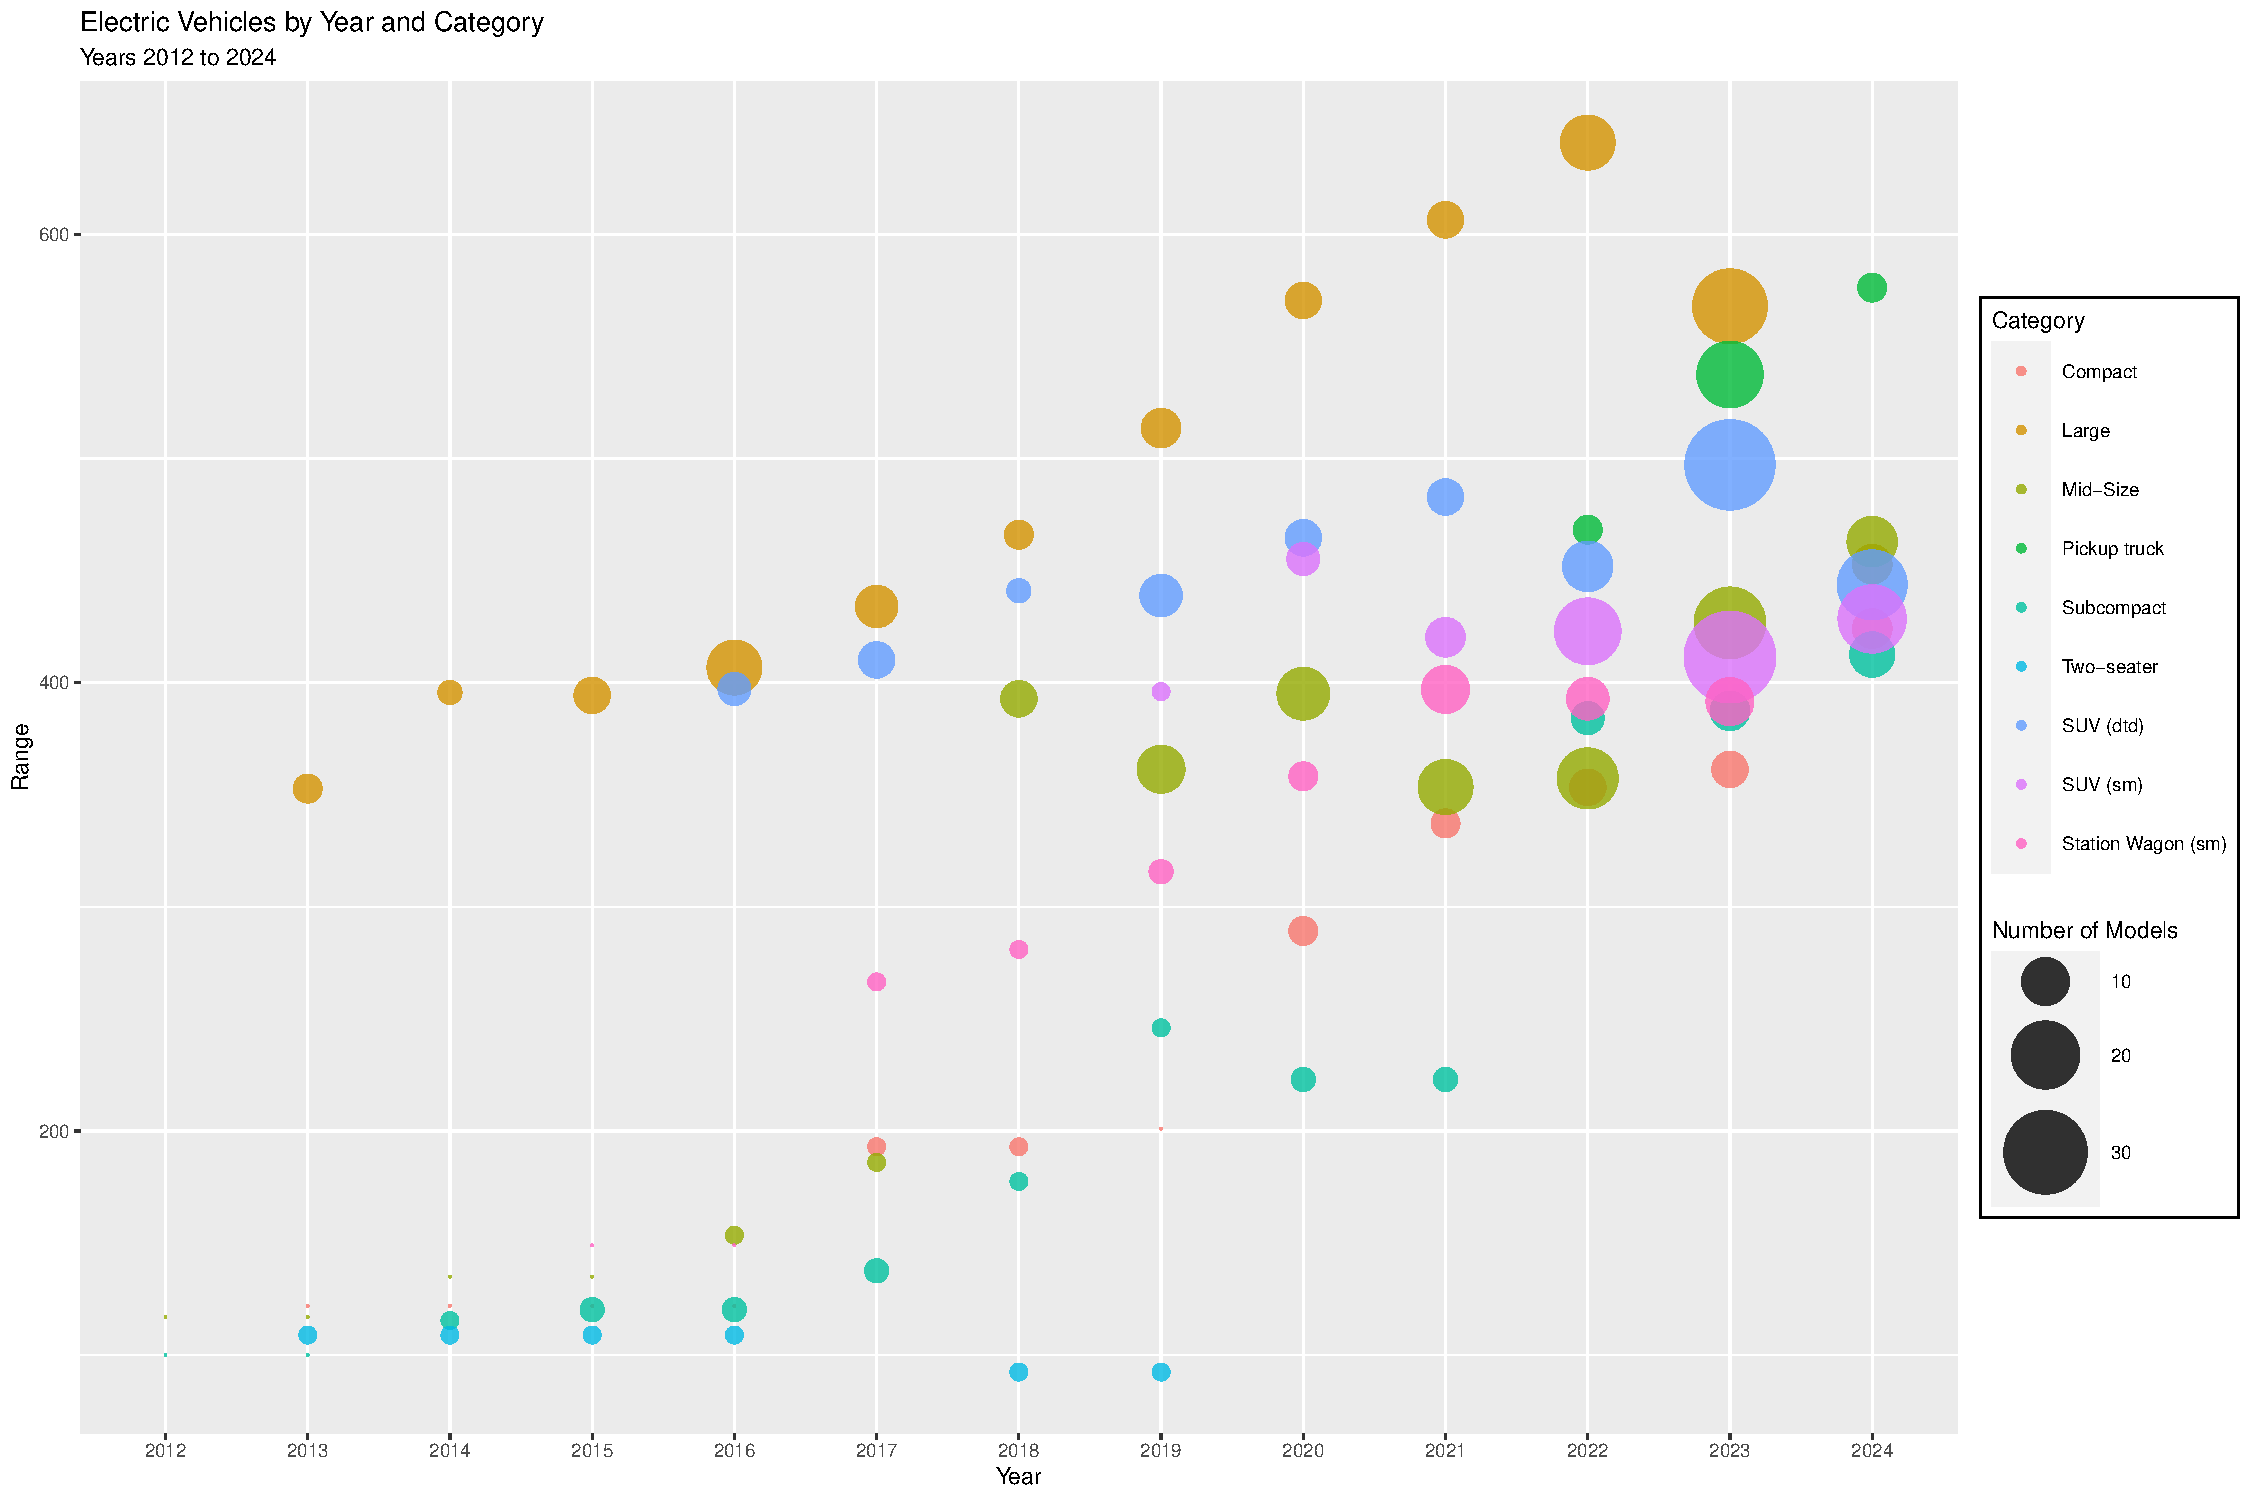
\includegraphics[width=\textwidth]{fuel.pointsSize.pdf}
\end{frame}

\begin{frame}[fragile]{Lines and Points Plot}
\footnotesize
\begin{Rcode}
e.clean %>% 
  filter(Year >= 2022 & Year <= 2023) %>%
  filter(Comb <= 4) %>%
  filter(Category != 'PL') %>%
  filter(Category != 'T') %>%
ggplot(aes(Comb, Range, 
           color=Category, 
           shape=Category, 
           linetype=Category)) +
  geom_line(size=1) + 
  geom_point(size=4) + 
\end{Rcode}
\end{frame}

\begin{frame}[fragile]{Lines and Points Plot \small [cont'd]}
Continued from previous slide \ldots
\footnotesize
\begin{Rcode}          
  scale_color_manual(values=c25, 
    labels=c('Compact', 'Large', 'Mid-Size', 
             'Subcompact', 'SUV (std)', 
             'SUV (sn)', 'Station Wagon (sm)')) + 
  scale_linetype(
    labels=c('Compact', 'Large', 'Mid-Size', 
             'Subcompact', 'SUV (std)', 
             'SUV (sm)', 'Station Wagon (sm)')) + 
  scale_shape(
    labels=c('Compact', 'Large', 'Mid-Size', 
             'Subcompact', 'SUV (std)', 
             'SUV (small)', 'Station Wagon (sm)')) + 
...
\end{Rcode}
\end{frame}


\begin{frame}{Lines and Points Plot}
  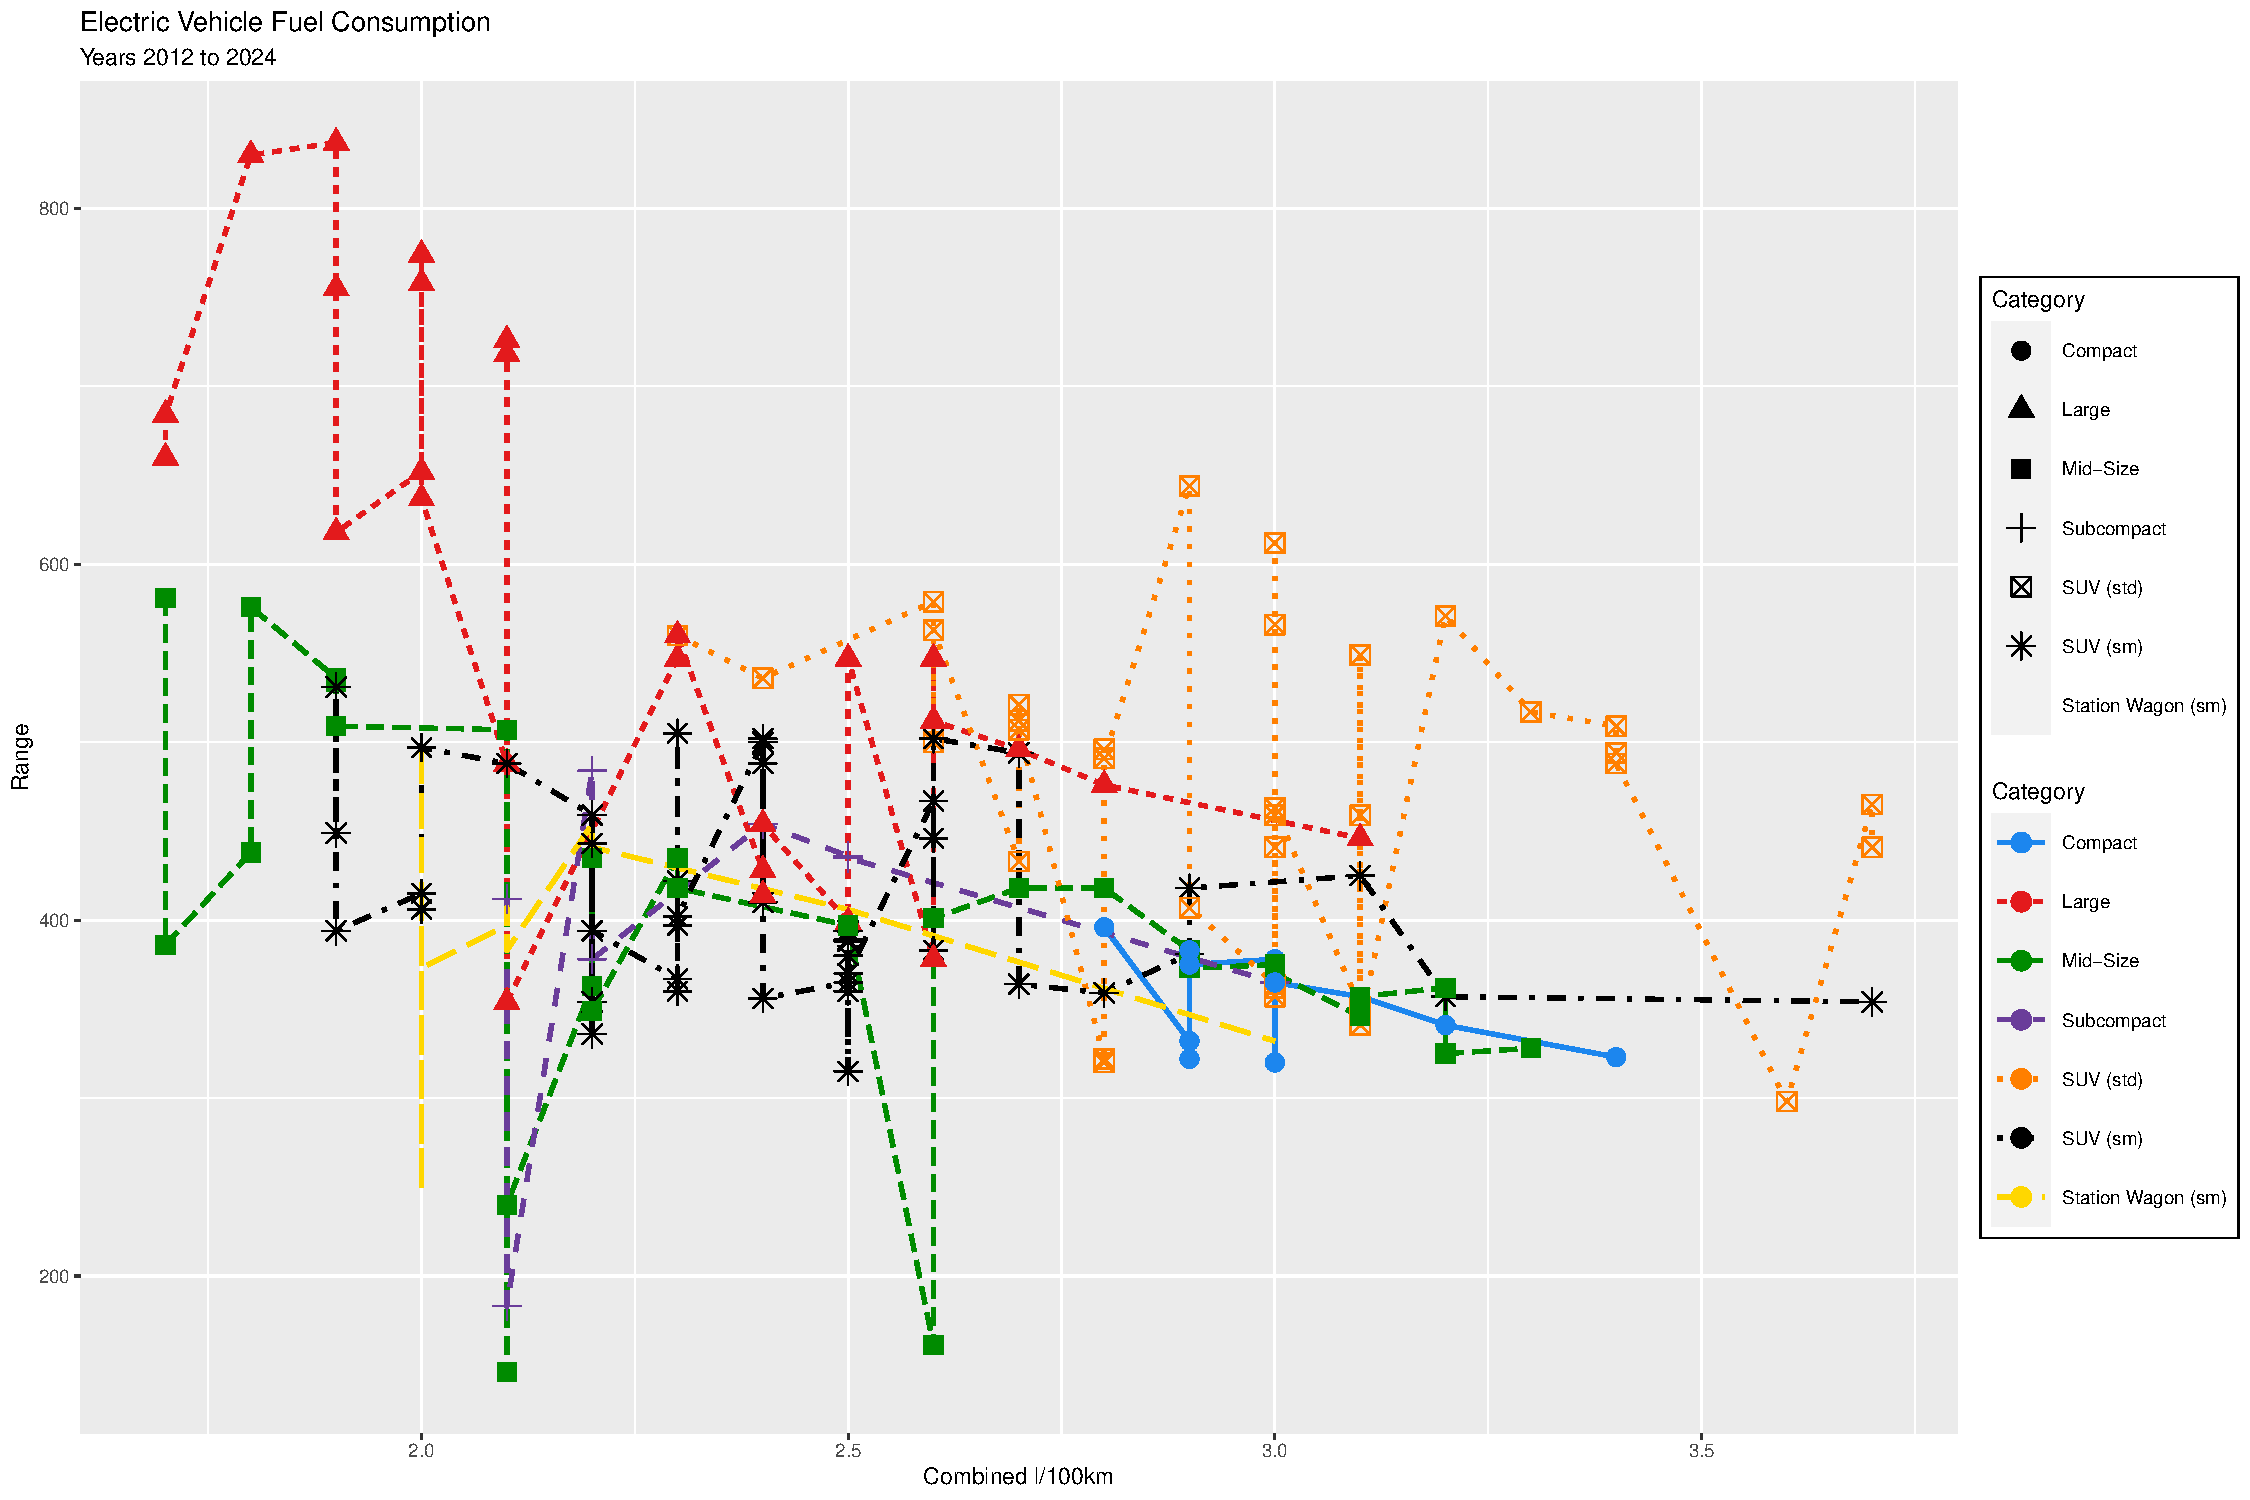
\includegraphics[width=\textwidth]{fuel.linesPoints.pdf}
\end{frame}

\begin{frame}[fragile]{Stepped Lines Plot}
\footnotesize
\begin{Rcode}
...
     geom_step(size=1) + 
... 
\end{Rcode}
\end{frame}

\begin{frame}{Stepped Lines Plot}
  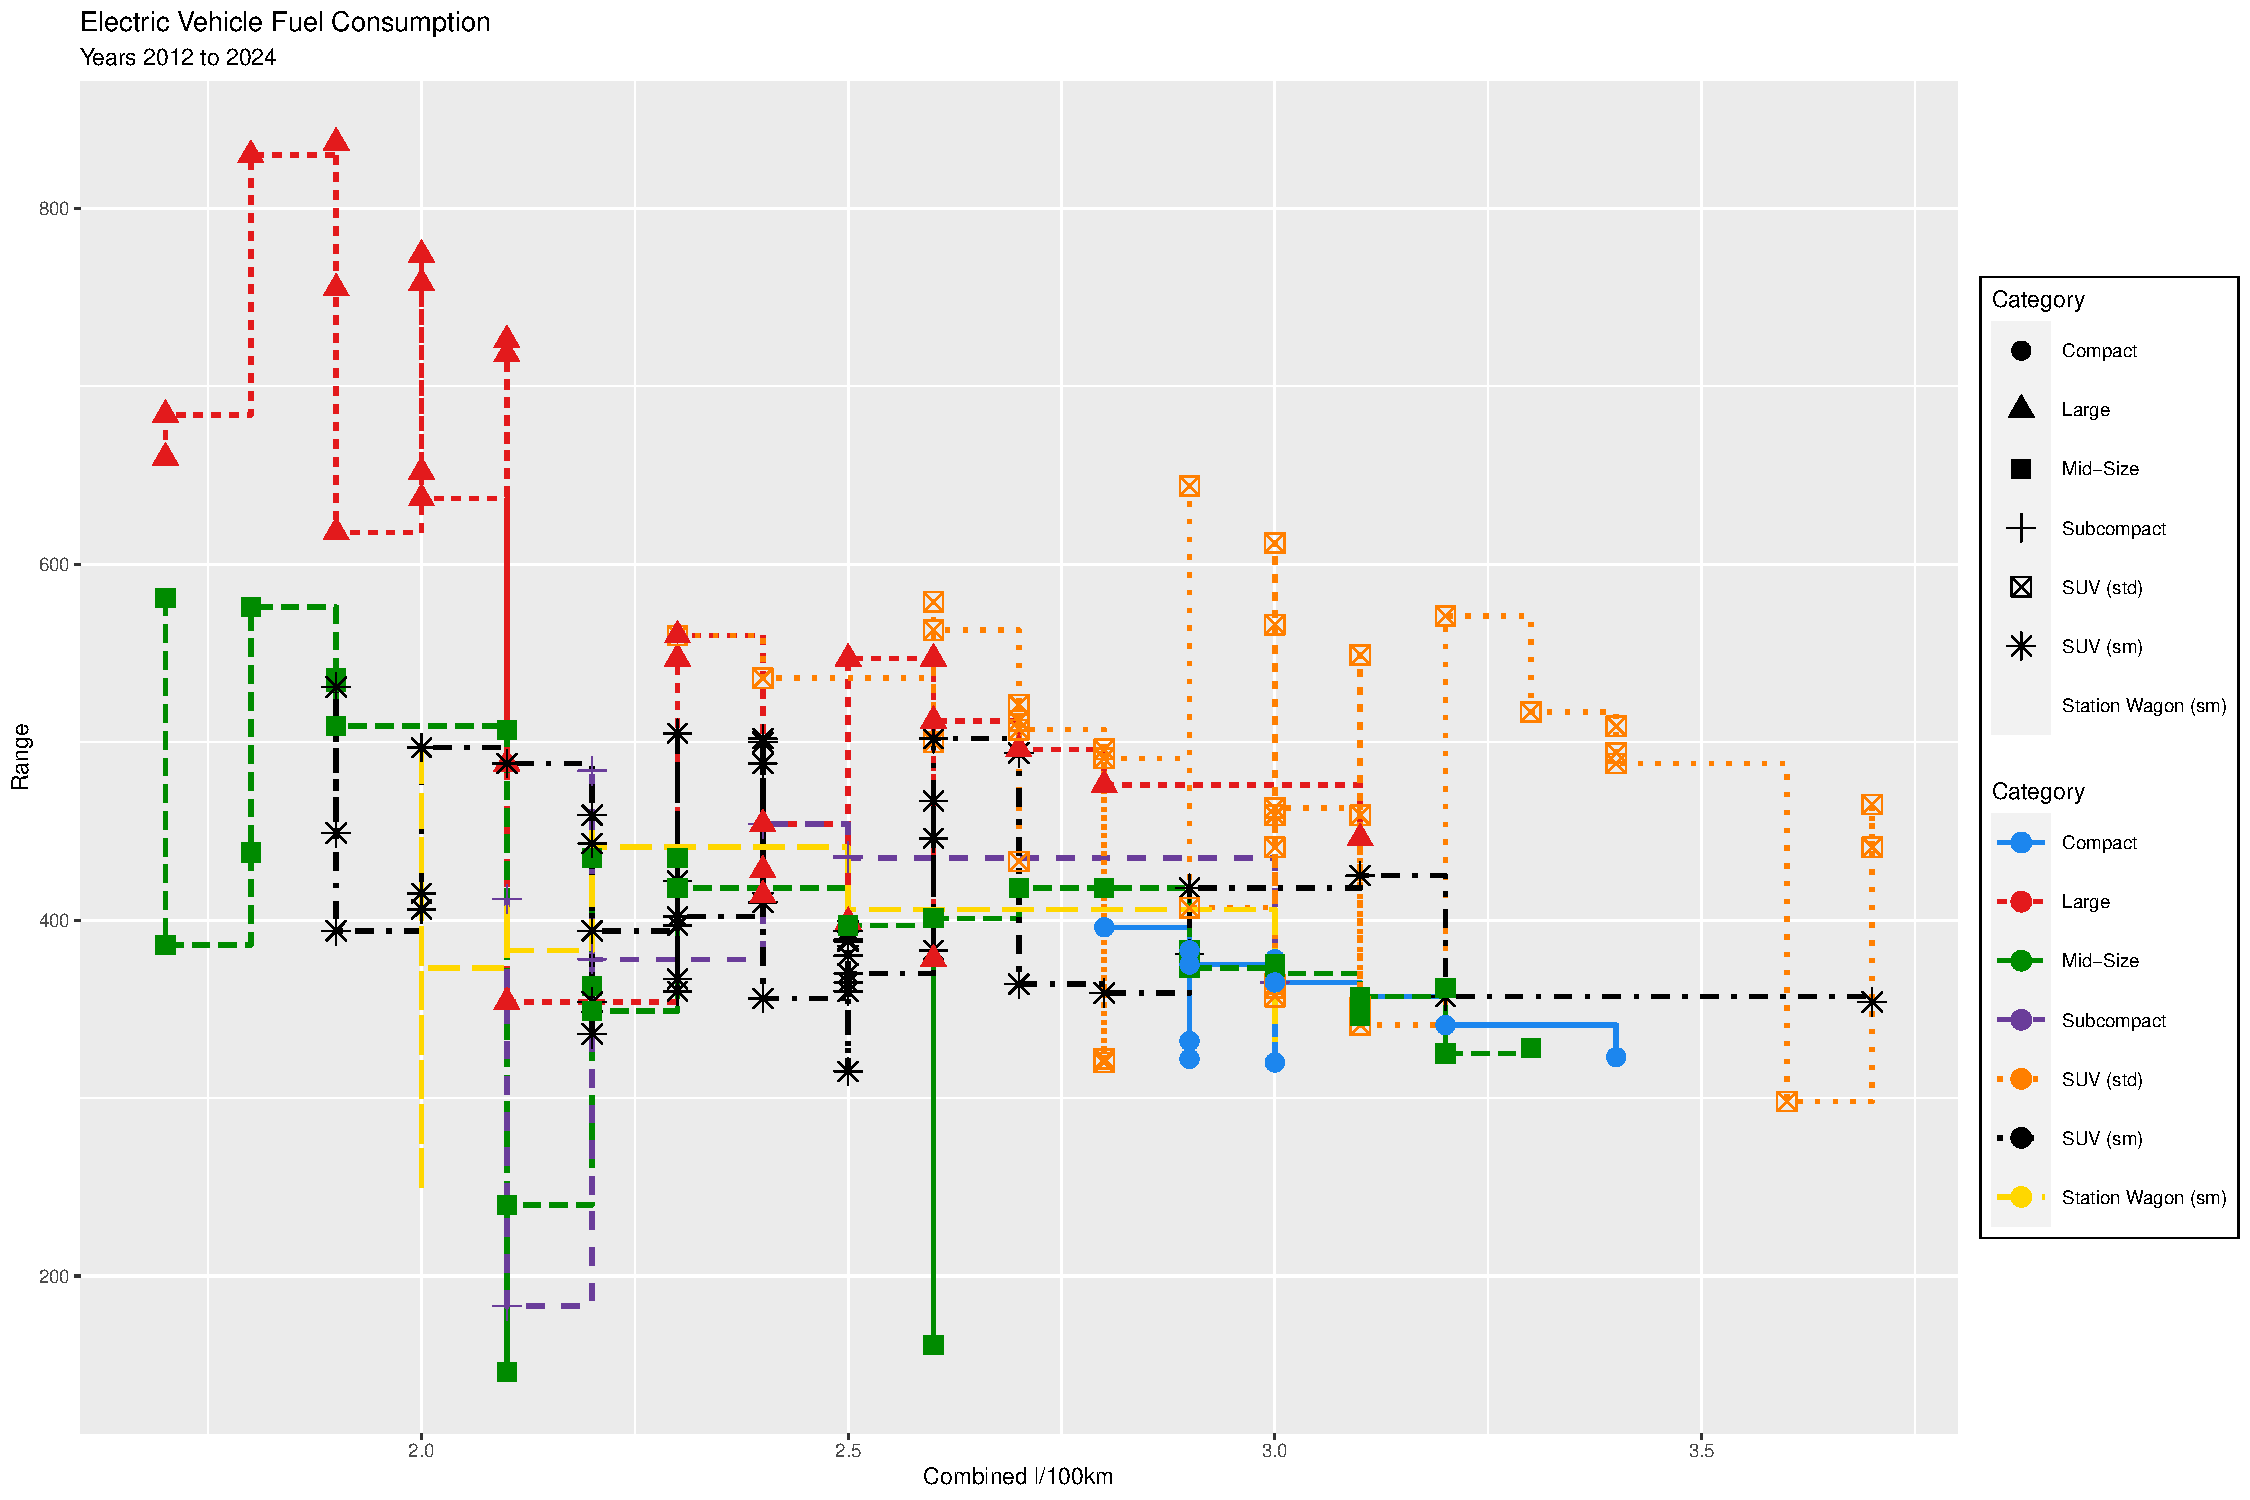
\includegraphics[width=\textwidth]{fuel.steps.pdf}
\end{frame}

\begin{frame}[fragile]{Pie Chart}
\footnotesize
\begin{Rcode}
e.clean %>% 
  filter(Year==2023) %>%
  group_by(Make) %>% summarize(totalcount = n()) %>%
  filter(totalcount >= 5) %>%
  ungroup() %>%
ggplot(aes(x='', y=totalcount, fill=Make)) +
  geom_bar(stat='identity', 
           color='black', size=0.25, width=1) + 
  coord_polar('y', direction=-1, start=0) +
  geom_text(aes(
     label=ifelse(totalcount >= 5,totalcount,'')), 
     color='lightgrey', 
     position = position_stack(vjust=0.5)) +
  scale_y_continuous(labels=NULL) + 
  scale_color_brewer(palette="Paired") +
  labs(x = '', y = '',  fill='Make', 
       title='Electric Vehicle Offerings by Make', 
       subtitle='2023, Makes with >= 5 models') +
  theme_void() +
  theme(legend.key.size=unit(1, 'cm'))
\end{Rcode}
\end{frame}

\begin{frame}{Pie Chart}
\centering
  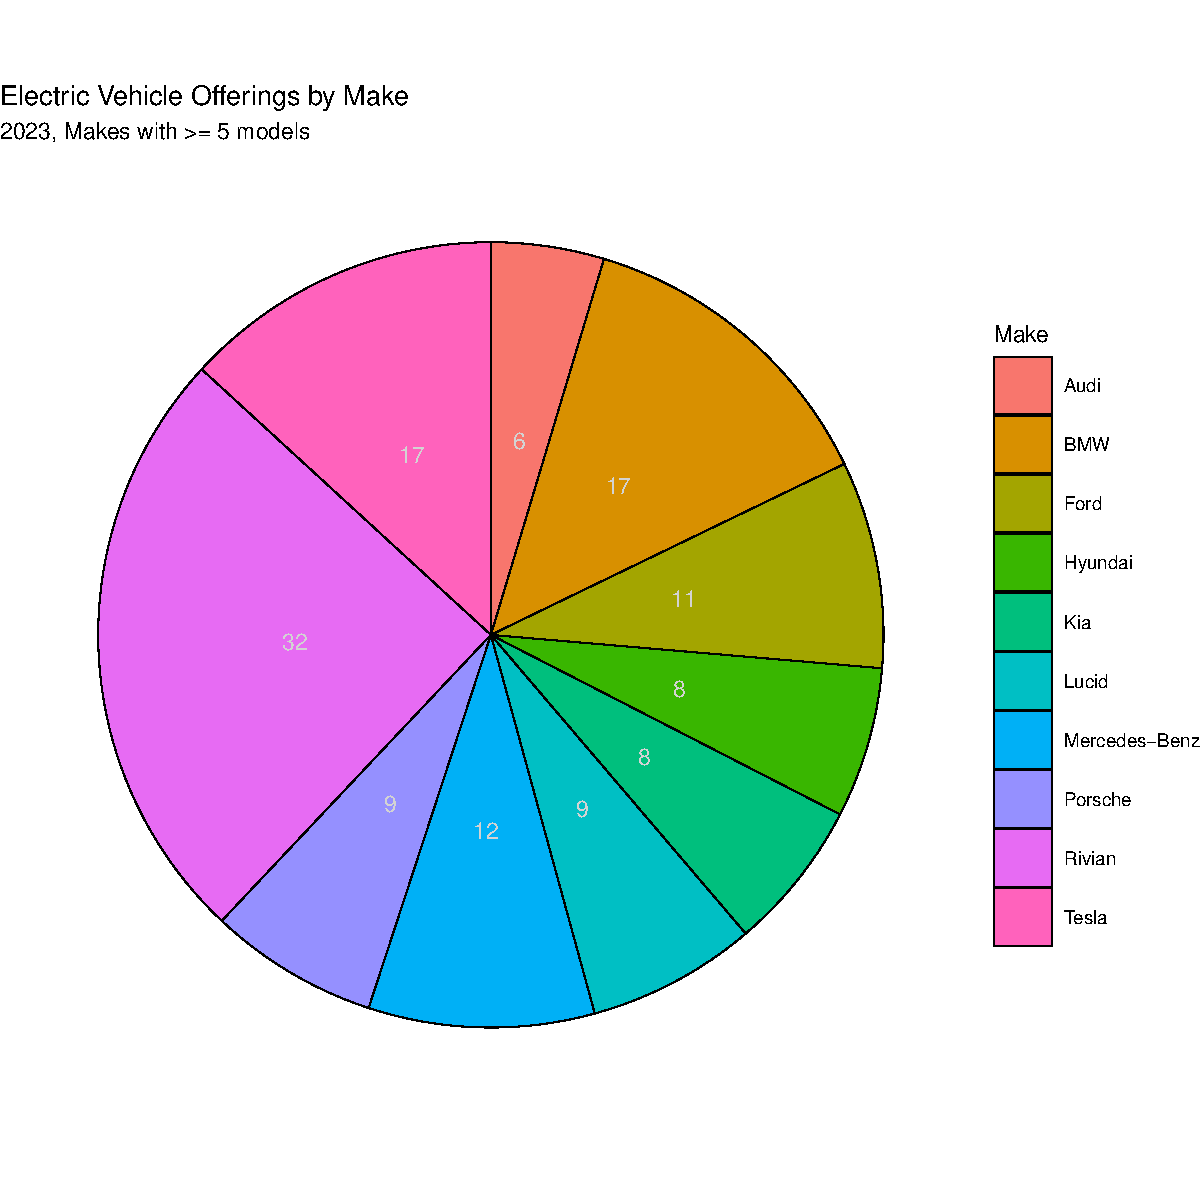
\includegraphics[width=.8\textwidth]{fuel.pie.pdf}
\end{frame}


\begin{frame}{Pie Charts (XKCD)}
  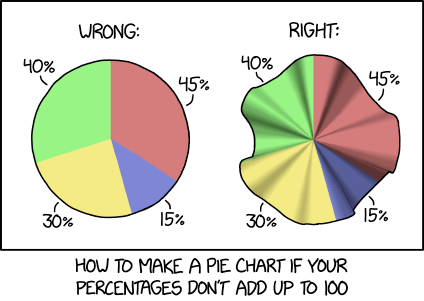
\includegraphics[width=\textwidth]{xkcd_pie_charts.png}
\end{frame}

\begin{frame}[fragile]{Donut Chart}
\footnotesize
\begin{minted}{R}
holesize <- 2

....

 ggplot(aes(x=holesize, y=totalcount, fill=Make)) +
   geom_col() + 
   xlim(c(0.2, holesize+0.5)) +
     
...

\end{minted}
\end{frame}

\begin{frame}{Donut Chart}
\centering
  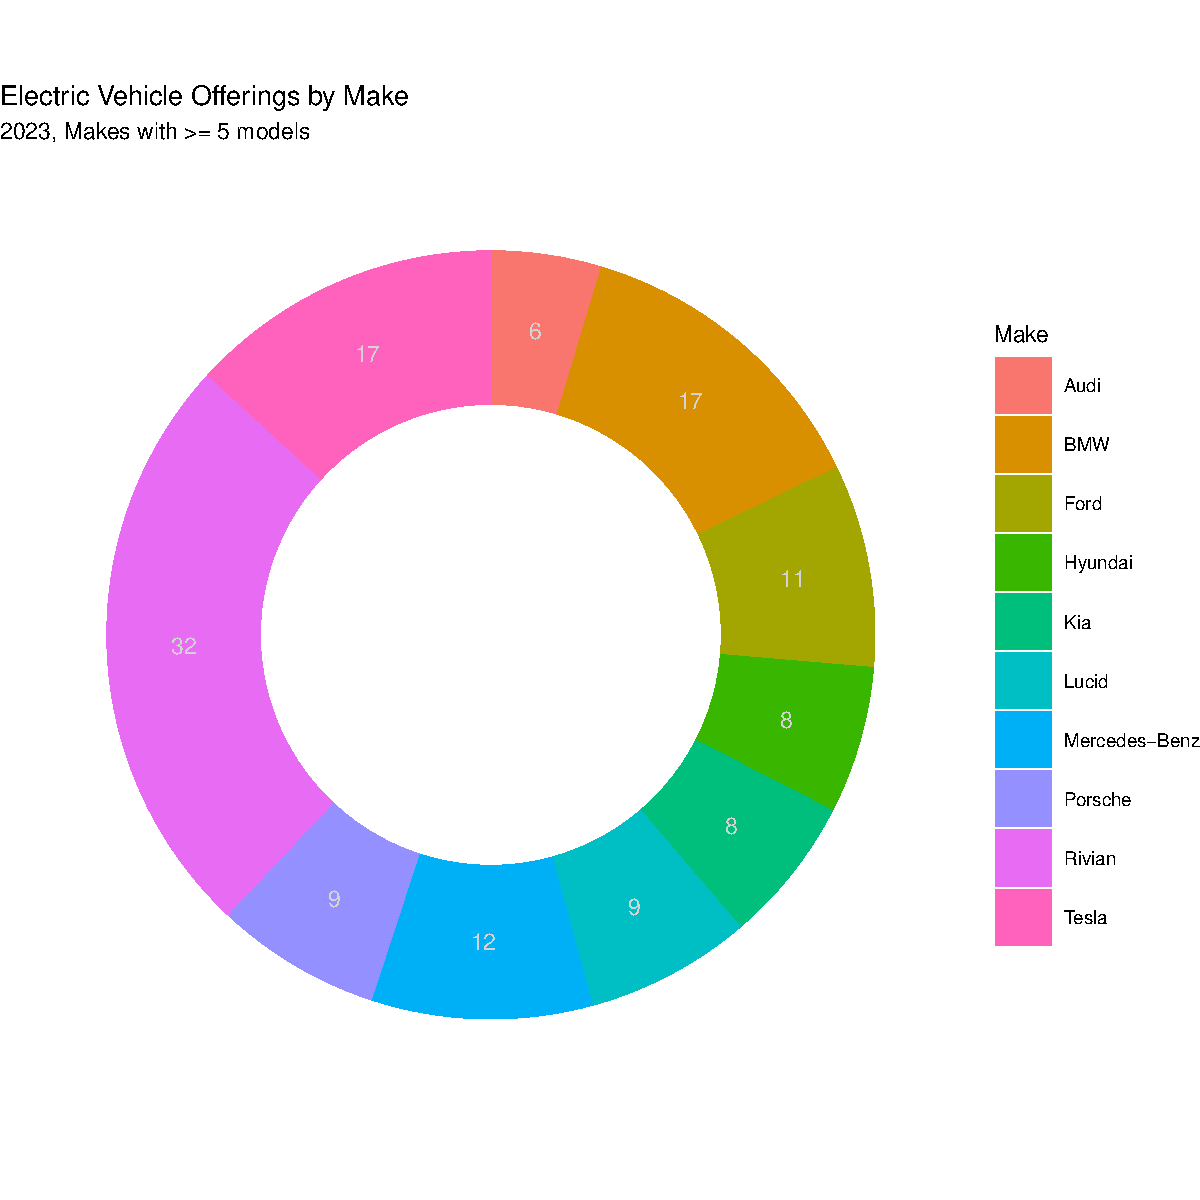
\includegraphics[width=.8\textwidth]{fuel.donut.pdf}
\end{frame}

\begin{frame}[fragile]{Radar Plot}
\footnotesize
\begin{Rcode}
e.clean %>% 
  filter(Year == 2023) %>% group_by(Make) %>%
  summarize(meanCity = 1/mean(City), 
            meanHwy = 1/mean(Hwy), 
            meanRange = mean(Range)/100, 
            nModels = n()) %>%
  filter(nModels >= 5) %>% ungroup() %>%
  select(-nModels) %>%
  mutate_at(vars(-Make), rescale) %>%
  ggradar(axis.labels=
             c('City', 'Highway', 'Range (100km)'), 
          values.radar='', 
          group.line.width=0.75, 
          group.point.size=3) +
     scale_color_ucscgb() +
  labs(x = '', y = '',  fill='Make', 
       title='Canadian Fuel Consumption Data', 
       subtitle='2023, Makes with more than 5 models')
\end{Rcode}
\end{frame}

\begin{frame}{Radar Plot}
\centering

  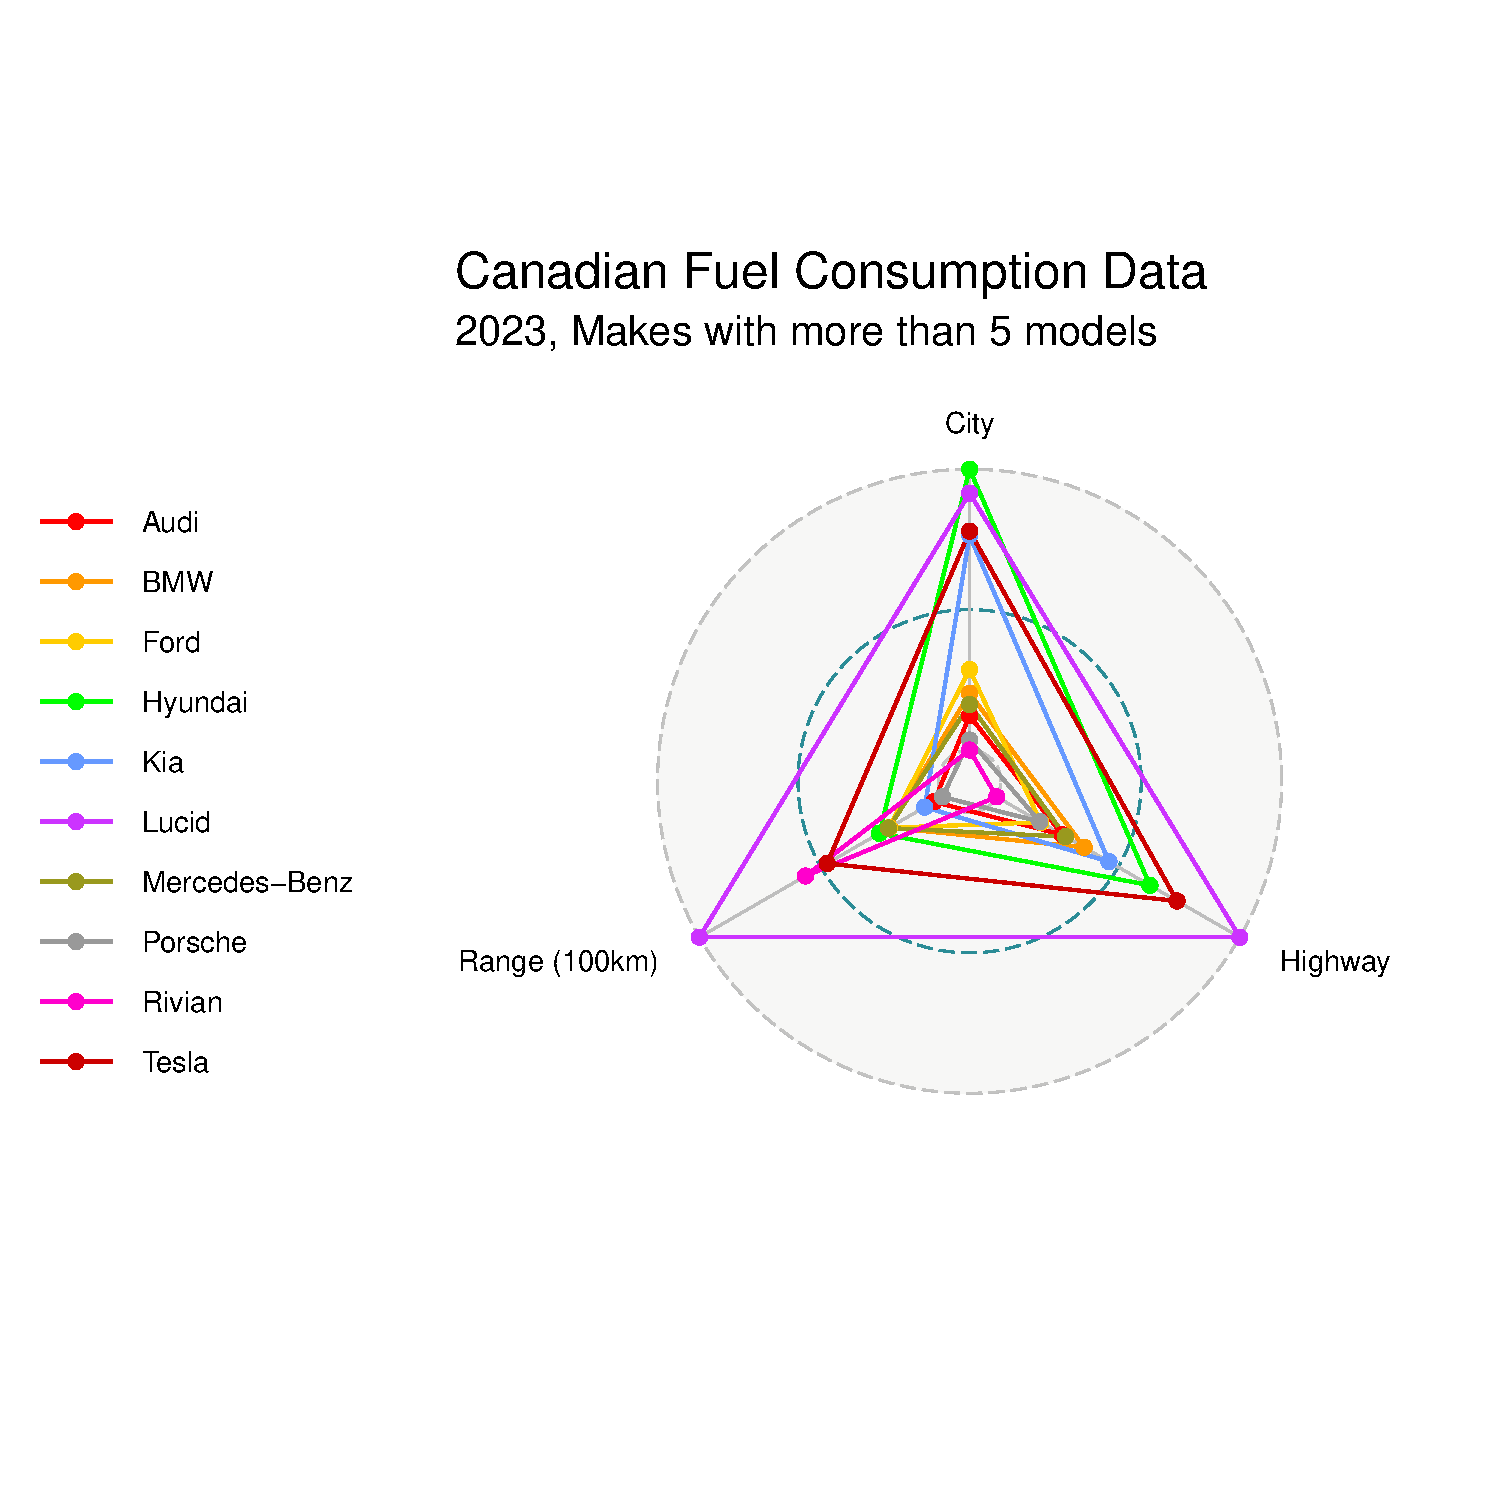
\includegraphics[width=.9\textwidth]{fuel.radar.pdf}
\end{frame}

\begin{frame}[fragile]{Lines with Multiple Axes}
\footnotesize
\begin{Rcode}
e.clean %>% 
   group_by(Year) %>%
   summarize(meanCity = mean(City), 
             meanHwy = mean(Hwy), 
             meanRange = mean(Range)) %>%
   ungroup() %>%
   mutate(meanRange2 = meanRange/100) %>%
\end{Rcode}
\end{frame}

\begin{frame}[fragile]{Lines with Multiple Axes}
\footnotesize
\begin{Rcode}
ggplot(aes(x=Year)) +
  scale_color_manual(name='Region', 
     values=c('Mean City' = 'red', 
              'Mean Highway' = 'blue', 
              'Mean Range' = 'orange')) +
  geom_line(aes(y=meanCity, color='Mean City')) + 
  geom_line(aes(y=meanHwy, color='Mean Highway')) +
  geom_line(aes(y=meanRange2, color='Mean Range')) +
  scale_y_continuous(labels=scales::comma, 
      name="Fuel Consumption\n(l/100km equiv)", 
      sec.axis=sec_axis(~ .*100, 
                        labels=scales::comma, 
                        name="Mean Range (km)")) + 
  scale_x_continuous(breaks=seq(from=2012,to=2024,by=1)) + 
  labs(x = 'Year', color='',
       title='Canadian Fuel Consumption Data', 
       subtitle='2012 to 2024') +
  theme(legend.key.size=unit(1.5, 'cm'), 
        axis.text.x = element_text(angle=45, hjust=1))
\end{Rcode}
\end{frame}

\begin{frame}{Lines with Multiple Axes}
  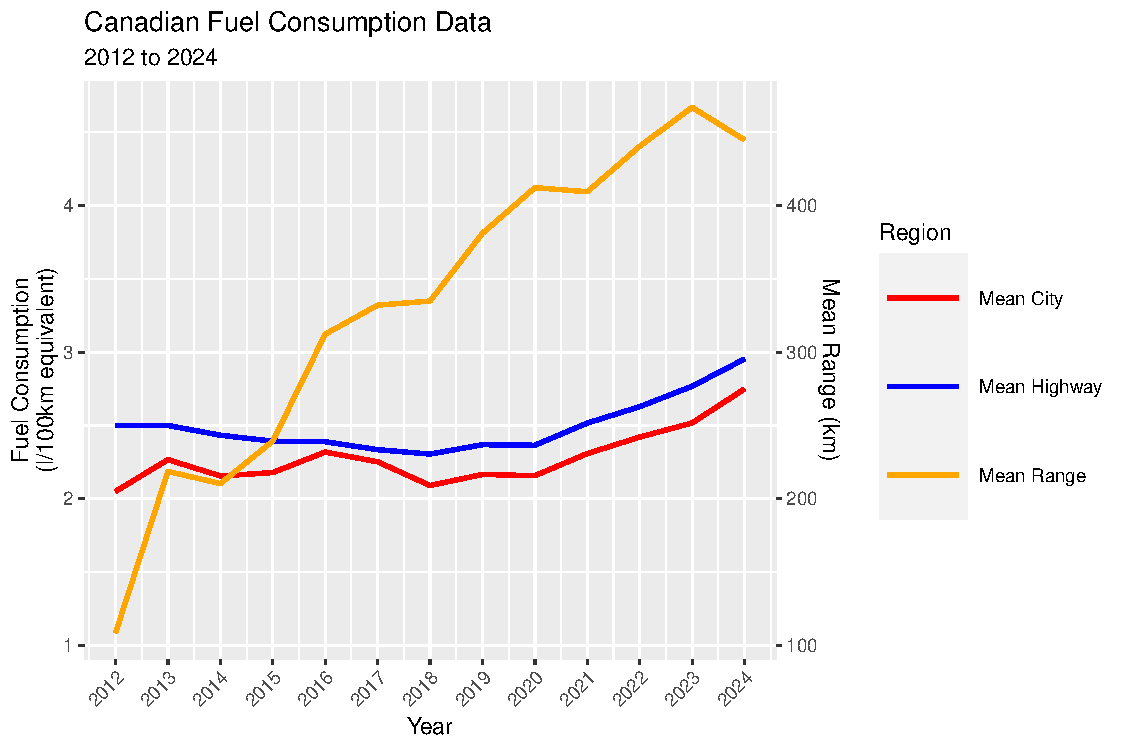
\includegraphics[width=\textwidth]{fuel.linesTwoScales.pdf}
\end{frame}

\begin{frame}[fragile]{Local Regression Smoothing Plot}
\footnotesize
\begin{Rcode}
e.clean %>% 
  ggplot(aes(Year, Range)) +
    geom_point() +
    geom_smooth() +
    scale_y_continuous(labels=scales::comma) + 
    labs(x = 'Year', color='', y = 'Mean Range (km)', 
         title='Canadian Fuel Consumption Data', 
         subtitle='2012 to 2024')
\end{Rcode}
\end{frame}

\begin{frame}{Local Regression Smoothing Plot}
  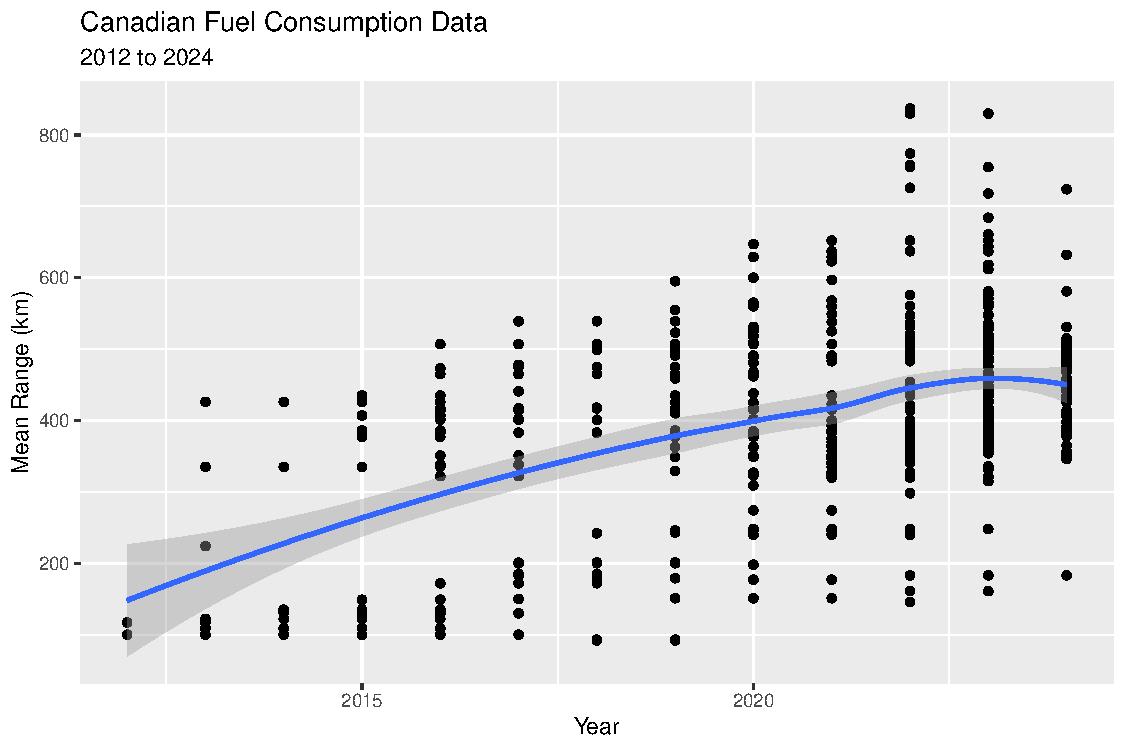
\includegraphics[width=\textwidth]{fuel.linesSmooth.pdf}
\end{frame}

\begin{frame}[fragile]{Local Regression Smoothing Plot (with range bar)}
\footnotesize
\begin{Rcode}
e.clean %>% 
  ggplot(aes(Year, Range)) +
    geom_point() +
    geom_smooth() +
    stat_summary(
       fun.data=mean_sdl, 
       fun.args=list(mult=1), 
       color='red', 
       geom="pointrange") +
    scale_y_continuous(labels=scales::comma) + 
    labs(x = 'Year', color='', y = 'Mean Range (km)', 
    title='Canadian Fuel Consumption Data', 
    subtitle='2012 to 2024')
\end{Rcode}
\end{frame}

\begin{frame}{Local Regression Smoothing Plot (with range bar)}
  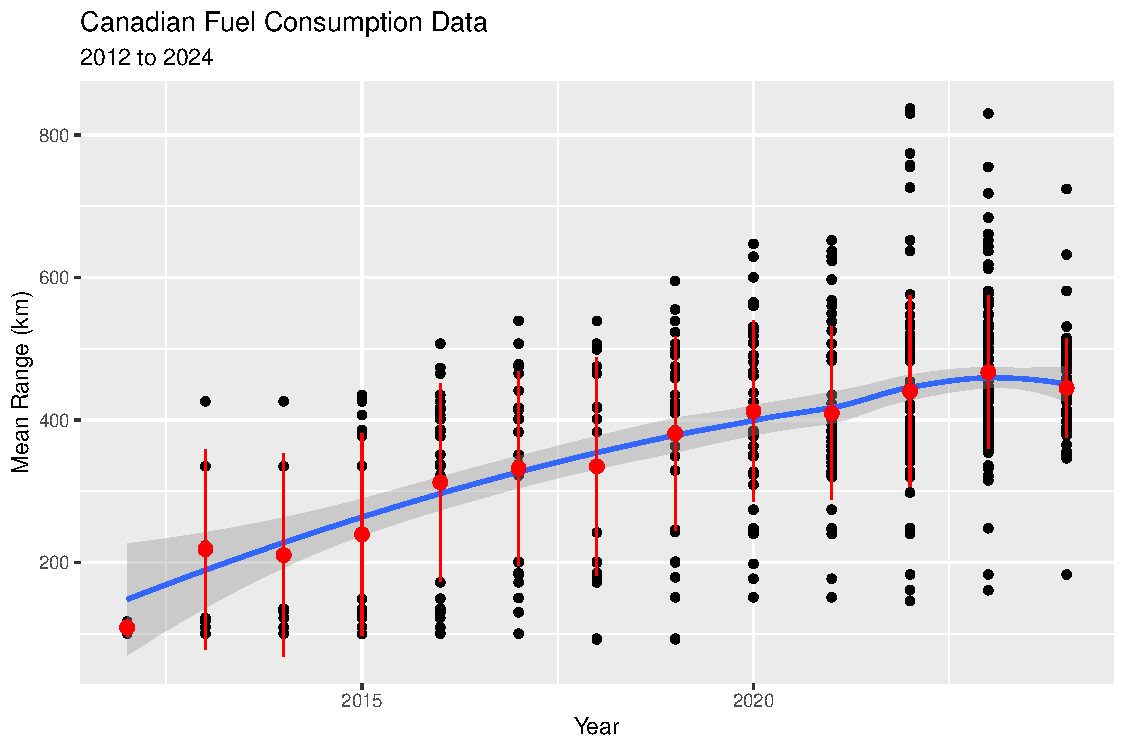
\includegraphics[width=\textwidth]{fuel.linesSmoothPointRange.pdf}
\end{frame}

\begin{frame}[fragile]{Local Regression Smoothing Plot (with error bars)}
\footnotesize
\begin{Rcode}
e.clean %>% 
  ggplot(aes(Year, Range)) +
    geom_point() +
    geom_smooth() +
    stat_summary(
        fun.data=mean_sdl, 
        fun.args=list(mult=1), 
        color='red', 
        geom="errorbar") +
    scale_y_continuous(labels=scales::comma) + 
    labs(x = 'Year', color='', y = 'Mean Range (km)', 
    title='Canadian Fuel Consumption Data', 
    subtitle='2012 to 2024')
\end{Rcode}
\end{frame}

\begin{frame}{Local Regression Smoothing Plot (with error bars)}
  \includegraphics[width=\textwidth]{fuel.linesSmoothErrorBar.pdf}
\end{frame}

\begin{frame}[fragile]{Local Regression Smoothing Plot (with cross bars)}
\footnotesize
\begin{Rcode}
e.clean %>% 
  ggplot(aes(Year, Range)) +
    geom_point() +
    geom_smooth() +
    stat_summary(
        fun.data=mean_sdl, 
        fun.args=list(mult=1), 
        color='red', 
        geom="crossbar",
        width=0.4) +
    scale_y_continuous(labels=scales::comma) + 
    labs(x = 'Year', color='', y = 'Mean Range (km)', 
    title='Canadian Fuel Consumption Data', 
    subtitle='2012 to 2024')
\end{Rcode}
\end{frame}

\begin{frame}{Local Regression Smoothing Plot (with cross bars)}
  \includegraphics[width=\textwidth]{fuel.linesSmoothCrossBar.pdf}
\end{frame}

\begin{frame}[fragile]{2D Density Plot}
\footnotesize
\begin{Rcode}
e.clean %>% 
  ggplot(aes(x=Hwy, y=City)) + 
    geom_point(color="black", size=1, 
               position='jitter') +
    geom_density_2d_filled(alpha=0.5) + 
    geom_density_2d(linewidth=0.25, colour='black') + 
    scale_x_continuous(labels=scales::comma) +
    labs(x = 'Highway Consumption\n(l/100km equiv)', 
         y = 'City Consumption\n(l/100km equiv)', 
         title='Density Plot-Fuel Consumption Ratings', 
         subtitle='Years 2015 to 2024') +
    theme(legend.position='none')
\end{Rcode}
\end{frame}

\begin{frame}{2D Density Plot}
  \includegraphics[width=\textwidth]{fuel.density2d.pdf}
\end{frame}

\begin{frame}[fragile]{2D Bin Plot}
\footnotesize
\begin{Rcode}
e.clean %>% 
  ggplot(aes(x=Hwy, y=City)) + 
    geom_point(color="black", size=1, 
               position='jitter') +
    geom_bin2d(alpha=0.5, bins=5) + 
    scale_x_continuous(labels=scales::comma) +
    labs(x = 'Highway Consumption\n(l/100km equiv)', 
         y = 'City Consumption\n(l/100km equiv)', 
         fill='Count', 
         title='Density Plot-Fuel Consumption Ratings', 
         subtitle='Years 2012 to 2024') 
\end{Rcode}
\end{frame}

\begin{frame}{2D Bin Plot}
  \includegraphics[width=\textwidth]{fuel.bin2d.pdf}
\end{frame}

\begin{frame}[fragile]{2D Hex Plot}
\footnotesize
\begin{Rcode}
e.clean %>% 
  ggplot(aes(x=Hwy, y=City)) + 
    geom_point(color="black", size=1, 
               position='jitter') +
    geom_hex(alpha=0.5, bins=5) + 
    scale_fill_distiller(palette=4, direction=-1) +
    scale_x_continuous(labels=scales::comma) +
    labs(x = 'Highway Consumption\n(l/100km equiv)', 
         y = 'City Consumption\n(l/100km equiv)', 
         fill='Count', 
         title='Density Plot-Fuel Consumption Ratings', 
         subtitle='Years 2012 to 2024') 
\end{Rcode}
\end{frame}

\begin{frame}{2D Hex Plot}
  \includegraphics[width=\textwidth]{fuel.hex2d.pdf}
\end{frame}

\begin{frame}[fragile]{3D Raster Plot}
\footnotesize
\begin{Rcode}
e.clean %>% 
  ggplot(aes(x=Hwy, y=City)) + 
    geom_point(color="black", size=0.5, 
               position='jitter') +
    geom_raster(aes(fill=Range), alpha=0.7, 
                interpolate=TRUE) + 
    scale_fill_distiller(palette=4, direction=-1) +
    scale_x_continuous(labels=scales::comma) +
    labs(x = 'Highway Consumption\n(l/100km equiv)', 
         y = 'City Consumption\n(l/100km equiv)', 
         fill='Range', 
         title='Raster Plot-Fuel Consumption Ratings', 
         subtitle='Years 2012 to 2024') 
\end{Rcode}
\end{frame}

\begin{frame}{3D Raster Plot}
  \includegraphics[width=\textwidth]{fuel.raster.pdf}
\end{frame}

\begin{frame}[fragile]{3D Raster Plot with Rug}
\footnotesize
\begin{Rcode}
e.clean %>% 
  ggplot(aes(x=Hwy, y=City)) + 
    geom_point(color="black", size=0.5, 
               position='jitter') +
    geom_raster(aes(fill=Range), alpha=0.7, 
                interpolate=TRUE) + 
    geom_rug(position='jitter') + 
    scale_fill_distiller(palette=4, direction=-1) +
    scale_x_continuous(labels=scales::comma) +
    labs(x = 'Highway Consumption\n(l/100km equiv)', 
         y = 'City Consumption\n(l/100km equiv)', 
         fill='Range', 
         title='Raster Plot-Fuel Consumption Ratings', 
         subtitle='Years 2012 to 2024') 
\end{Rcode}
\end{frame}

\begin{frame}{3D Raster Plot (with rug)}
  \includegraphics[width=\textwidth]{fuel.raster.rug.pdf}
\end{frame}

\begin{frame}{Hands-On Exercises}
\footnotesize
Using the Pagila database data from \url{https://evermann.ca/busi4720/rentals.csv}, create
\begin{enumerate}
   \item A histogram and/or density chart of film length by film category
   \item A column chart of the mean rental payments for films by film category
   \begin{itemize}
	  \footnotesize
      \item Add error bars to this chart
   \end{itemize}
   \item A scatter plot of total rental payments by year and week
   \begin{itemize}
	  \footnotesize
      \item Add a local regression line to this plot
   \end{itemize}
   \item A pie or donut chart of rental counts by film rating
\end{enumerate}
\textbf{Tips:}
\begin{itemize}
\item The \texttt{read.csv()} function can read from a URL
\item The data is de-normalized, use the \texttt{unique()} function to get accurate film counts for exercise 1
\item Use the \texttt{year()} and \texttt{week()} functions from the \texttt{lubridate} package (another package of the Tidyverse set)
\end{itemize}
\end{frame}


\end{document}
